\subsection{Chapter 10 - Rotational dynamics}

\subsubsection{Overview}\label{chap:rotationaldynamics}

In this Chapter, we use Newton's Second Law to develop a formalism to describe how objects rotate. In particular, we will introduce the concept of torque which plays a similar role to that of force in non-rotational dynamics. We will also introduce the concept of moment of inertia to describe how objects resist rotational motion.

\begin{framed}
\textbf{Learning Objectives}\\
\begin{itemize}
\item Understand how to use vector quantities for describing the kinematics of rotations.
\item Understand how to use torque to determine the angular acceleration of an object.
\item Understand conditions for static and dynamic equilibrium.
\item Understand how to determine the moment of inertia of an object.
\end{itemize}
\end{framed}

\begin{framed}
\textbf{Think About It}\\
A construction worker would like to lift one end of a heavy block from the ground using a bar propped against a rock on the ground as a lever. Should he place the rock close or far from the block to make it easier to lift the block?\}

\begin{enumerate}
\item It will be easier to lift the block if the rock is close to the block.
\item It will be easier to lift the block if the rock is far from the block.
\item It does not matter where he places the rock, as long as the bar is short.
\item It does not matter where he places the rock, as long as the bar is long.
\end{enumerate}

\begin{framed}
\textbf{Answer}\\
\begin{enumerate}
\item
\end{enumerate}
\end{framed}
\end{framed}

\subsubsection{Rotational kinematic vectors}

\begin{framed}
\textbf{Review}\\
Before proceeding, you may wish to review:

\begin{itemize}
\item Section~\ref{sec:momentumandcm:circularmotion} on kinematics for circular motion.
\item Section~\ref{sec:Vectors:vectorproduct} on the vector product.
\item Section~\ref{sec:Vectors:rotationalmotion} on axial vectors and their use in defining rotational quantities.
\end{itemize}
\end{framed}

\paragraph{Scalar rotational kinematic quantities}

Recall that we can describe the motion of a particle along a circle of radius, $R$, by using its angular position, $\theta$, its angular velocity, $\omega$, and its angular acceleration, $\alpha$. With a suitable choice of coordinate system, the angular position can be defined as the angle made by the position vector of the particles, $\vec r$, and the $x$ axis of a coordinate system whose origin is the centre of the circle, as shown in Figure~\ref{fig_rotationaldynamics_vcircle}.

\begin{figure}[!htbp]
\centering
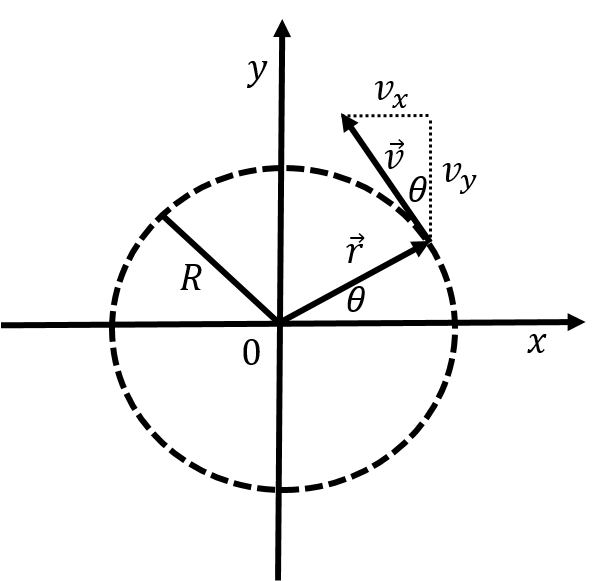
\includegraphics[width=0.375\linewidth]{files/vcircle-84a2b9eb9617dd4b79c73a0e096f77a8.png}
\caption[]{Angular position for a particle moving around the $z$ axis (out of the page), along a circle of radius $R$ with a centre at the origin.\}}
\label{fig_rotationaldynamics_vcircle}
\end{figure}

The angular velocity, $\omega$, is the rate of the change of the angular position, and the angular acceleration, $\alpha$, is the rate of change of the angular velocity:
\begin{align*}
\omega &= \frac{d}{dt}\theta \\
\alpha &= \frac{d}{dt}\omega
\end{align*}
If the angular acceleration is constant, then angular velocity and position as a function of time are given by:
\begin{align*}
\omega(t) = \omega_0+\alpha t\\
\theta(t) = \theta_0+\omega_0 t+\frac{1}{2}\alpha t^2
\end{align*}
where $\theta_0$ and $\omega_0$ are the angular position and velocity, respectively, at $t=0$.

We can also describe the motion of the particle in terms of ``linear'' quantities (as opposed to ``angular'' quantities) along a one-dimensional axis that is curved along the circle. If $s$ is the distance along the circumference of the circle, measured counter-clockwise from where the circle intersects the $x$ axis, then it is related to the angular displacement:
\begin{align*}
s = R\theta
\end{align*}
if $\theta$ is expressed in radians. Similarly, the linear velocity along the $s$ axis, $v_s$, and the corresponding acceleration, $a_s$, are given by:
\begin{align*}
v_s &= \frac{ds}{dt} =\frac{d}{dt}R\theta = R\omega\\
a_s&= \frac{dv}{dt} =\frac{d}{dt}R\omega = R\alpha
\end{align*}
where the radius of the circle, $R$, is a constant that can be taken out of the time derivatives. For motion along a circle, the velocity vector, $\vec v$, of the particle is always tangent to the circle (\href{\#fig:rotationaldynamics:vcircle}{}), so $v_s$ corresponds to the speed of the particle. The acceleration vector, $\vec a$, is in general not tangent to the circle; $a_s$ represents the component of the acceleration vector that is tangent to the circle. If $a_s=0$, then $\alpha=0$, and the particle is moving with a constant speed (uniform circular motion), and the acceleration vector points towards the centre of the circle.

\begin{framed}
\textbf{Checkpoint}\\
Which of the following statements correctly describes the speeds at points $A$ and $B$ on the disk rotating about an axis through its centre, as illustrated in Figure~\ref{fig_rotationaldynamics_rotatingdisk}?

\begin{enumerate}
\item Both points A and B have the same angular and linear speeds.
\item Both points A and B have the same linear speed but they have different angular speeds.
\item Both points A and B have the same angular speed but they have different linear speeds.
\end{enumerate}

\begin{figure}[!htbp]
\centering
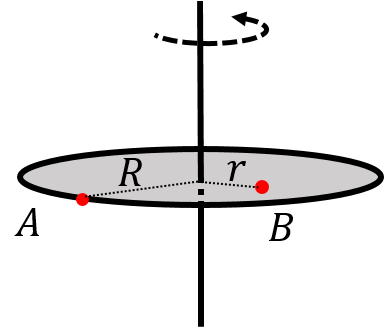
\includegraphics[width=0.375\linewidth]{files/rotatingdisk-fb0502378e225f6c9e0e3f469178fbe1.png}
\caption[]{Two points at different radii on a rotating disk.
:align: center}
\label{fig_rotationaldynamics_rotatingdisk}
\end{figure}

\begin{framed}
\textbf{Answer}\\
\begin{enumerate}[resume]
\item
\end{enumerate}
\end{framed}
\end{framed}

\paragraph{Vector rotational kinematic quantities}

In the previous section, we defined angular quantities to describe the motion of a particle about the $z$ axis along a circle of radius $R$ that lies in the $xy$ plane. By using vectors, we can define the angular quantities for rotation about an \textbf{axis that can point in any direction}. Given an axis of rotation, the path of any particle rotating about that axis can be described by a circle that lies in the plane perpendicular to that axis of rotation, as illustrated in Figure~\ref{fig_rotationaldynamics_axis}.

\begin{figure}[!htbp]
\centering
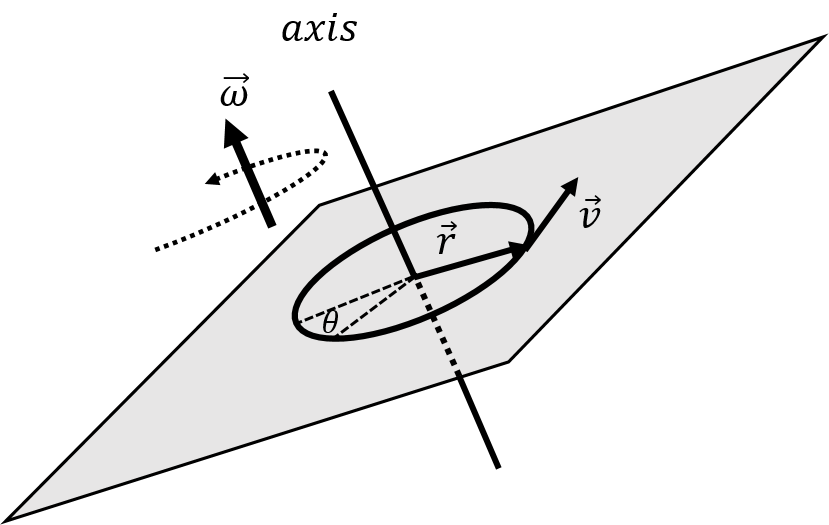
\includegraphics[width=0.375\linewidth]{files/axis-75d811d50a499c9ab25572740f7803f0.png}
\caption[]{Defining the vector $\vec r$ and the angular velocity, $\vec \omega$ for a particle with velocity $\vec v$ rotating about an axis in a general direction.}
\label{fig_rotationaldynamics_axis }
\end{figure}

We define the vector, $\vec r$, for a particle to be the vector that goes from the axis of rotation to the particle and is in a plane perpendicular to the axis of rotation, as in Figure~\ref{fig_rotationaldynamics_axis}. Given the velocity vector of the particle, $\vec v$, we define its angular velocity vector, $\vec\omega$, \textbf{about the axis of rotation}, as:
\begin{equation}
\boxed{\vec \omega = \frac{1}{r^2} \vec r \times \vec v}
\end{equation}
The angular velocity vector is perpendicular to both the velocity vector and the vector $\vec r$, since it is defined as their cross-product. Thus, the \textbf{angular velocity vector is co-linear with the axis of rotation}. By using the angular velocity vector, we can specify \textbf{the direction of the axis of rotation as well as the direction in which the particle is rotating about that axis}. The direction of rotation is given by the right hand rule for axial vectors: when you point your thumb in the same direction as the angular velocity vector, the direction of rotation is the direction that your fingers point when you curl them, as illustrated in Figure~\ref{fig_rotationaldynamics_hand}.

\begin{figure}[!htbp]
\centering
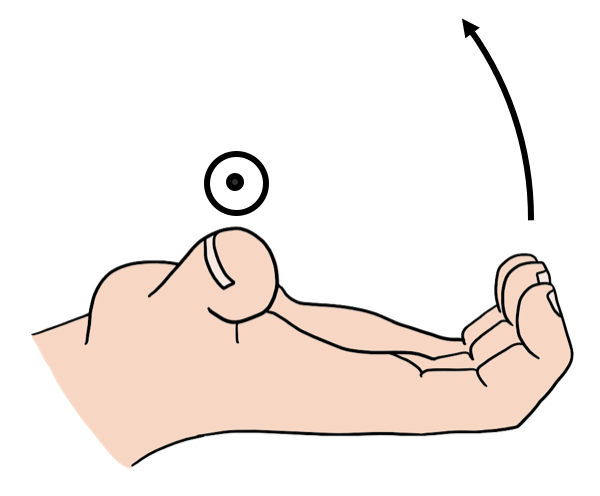
\includegraphics[width=0.375\linewidth]{files/righthandruleaxial-b9e11f05b12444487db6c9f4d42438c9.png}
\caption[]{Using the right hand rule for axial vectors. In this case, the direction of rotation is counter clockwise when looking at the page (the direction that the fingers curl), so the rotation vector points out of the page (the direction of the thumb).}
\label{fig_rotationaldynamics_hand}
\end{figure}

This definition of the angular velocity is consistent with the description from the previous section for motion about a circle of radius $R$ that lies in the $xy$ plane, as in Figure~\ref{fig_rotationaldynamics_vcircle}. In that case, the magnitude of the angular velocity is given by:
\begin{align*}
\omega &=\frac{1}{r^2} || \vec r \times \vec v||= \frac{1}{r^2}r v\sin\phi= \frac{v}{R}\\
\therefore v &= R\omega
\end{align*}
where $\phi$ is the angle between the vectors $\vec r$ and $\vec v$ ($90{\degree}$ for motion around a circle). The direction of the angular velocity in Figure~\ref{fig_rotationaldynamics_vcircle} is in the positive $z$ direction, which corresponds to counter-clockwise rotation about the $z$ axis.

\begin{framed}
\textbf{Checkpoint}\\
You push on the right-hand side of a door to open it, as the door's hinges are on the left. The angular velocity vector of the door is:

\begin{enumerate}
\item Upwards
\item Downwards
\item Forwards
\item Backwards
\end{enumerate}

\begin{framed}
\textbf{Answer}\\
\begin{enumerate}
\item
\end{enumerate}
\end{framed}
\end{framed}

One can always define an angular velocity vector \textbf{relative to a point of rotation}, even if the particle is not moving along a circle. If we define the vector $\vec r$ to be the vector from the point of rotation to the particle, then the angular velocity vector describes the motion of the particle as if it were instantaneously moving in a circle centred at the point of rotation, in a plane given by the vectors $\vec r$ and $\vec v$.

Consider, for example, the particle in Figure~\ref{fig_rotationaldynamics_vline} which is moving in a straight line with a velocity vector in the $xy$ plane at a position $\vec r$ relative to the origin. We can define its angular velocity vector relative to the origin, which will be in the positive $z$ direction.

\begin{figure}[!htbp]
\centering
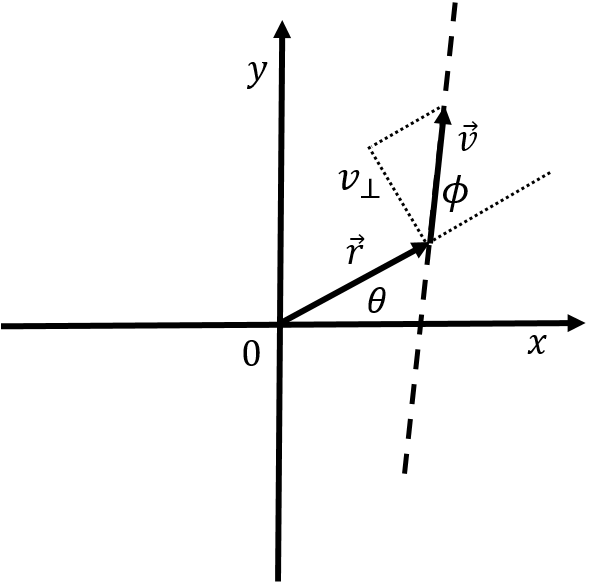
\includegraphics[width=0.375\linewidth]{files/vline-dade52a6a4387571d252280093213e03.png}
\caption[]{Angular position for a particle moving in a straight line.}
\label{fig_rotationaldynamics_vline}
\end{figure}

The angular velocity describes the motion of the particle as if it were \textbf{instantaneously moving along a circle of radius $r$ centred about the origin}. The angular velocity is related to the component of $\vec v$, $v_\perp$, that is perpendicular to $\vec r$ (which is the component tangent to the circle of radius $r$, in Figure~\ref{fig_rotationaldynamics_vline}:
\begin{equation}
||\vec \omega|| = \frac{1}{r^2} || \vec r \times \vec v||=\frac{v\sin\phi}{r}= \frac{v_\perp}{r}
\end{equation}
where $\phi$ is the angle between $\vec r$ and $\vec v$.

Similarly, we can define the angular acceleration vector, $\vec \alpha$, about an axis of rotation:
\begin{equation}
\vec \alpha = \frac{1}{r^2}\vec r \times \vec a
\end{equation}
where $\vec a$ is the particle's acceleration vector,  and $\vec r$ is the vector from the axis of rotation to the particle. The direction of the angular acceleration is co-linear with the axis of rotation and the right-hand rule gives the rotational direction of the angular acceleration. We can also define the angular acceleration about a point; in that case, the direction of the vector will define an instantaneous axis of rotation about a circle of radius $r$ centred at the point as well as the direction of the angular acceleration about that axis.

Finally, we can define an angular displacement vector, $\vec \theta$, relative to an axis of rotation. The direction of the angular displacement vector will be co-linear with the axis of rotation, its direction will indicate the direction of rotation about that axis, and its magnitude (in radians) will correspond to the angular displacement (as shown in Figure~\ref{fig_rotationaldynamics_axis}). We can only relate the angular displacement vector to an infinitesimal linear displacement vector, $d\vec s$, since the position vector $\vec r$ from the axis of rotation will be different at each end of the displacement vector if the displacement is large. The infinitesimal angular displacement vector that corresponds to an infinitesimal displacement vector, $d\vec s$, is defined as:
\begin{align*}
d\vec \theta &= \frac{1}{r^2} \vec r \times d\vec s\\
\end{align*}

\begin{framed}
\textbf{Checkpoint}\\
Which statement is correct regarding an ant on a disk that is rotating slower and slower as illustrated in Figure~\ref{fig:rotationaldynamics:ant}?

\begin{figure}[!htbp]
\centering
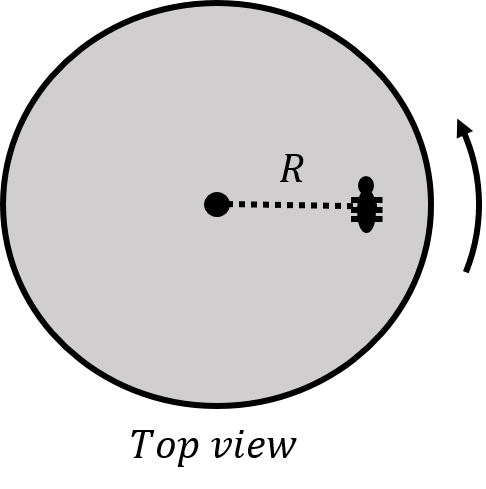
\includegraphics[width=0.375\linewidth]{files/ant-462cf685aaf5841e43d592702e783193.png}
\caption[]{An ant on a disk.}
\label{fig:rotationaldynamics:ant}
\end{figure}

\begin{enumerate}
\item The angular velocity points into the page and the angular acceleration points out of the page.
\item Both the angular velocity and acceleration point into the page.
\item Both the angular velocity and acceleration point out of the page.
\item The angular acceleration points into the page and the angular velocity points out of the page.
\end{enumerate}

\begin{framed}
\textbf{Answer}\\
\begin{enumerate}[resume]
\item
\end{enumerate}
\end{framed}
\end{framed}

The instantaneous angular velocity vector is the rate of change of the angular displacement vector:
\begin{align*}
\vec\omega &= \frac{d\vec \theta}{dt} = \frac{d}{dt} \frac{1}{r^2} \vec r \times d\vec s = \frac{1}{r^2} \vec r \times \vec v_s
\end{align*}
where $\vec v_s$ is the (instantaneous) tangential velocity around the circle (i.e. the component of the velocity $\vec v$ that is perpendicular to $\vec r$). The angular acceleration vector is the rate of change of the angular velocity vector:
\begin{align*}
\vec\alpha = \frac{d}{dt} \vec \omega
\end{align*}

Given the angular kinematic quantities, the related linear quantities at a position $\vec r$ from the axis of rotation are given by:
\begin{equation}
d\vec s &= d\vec\theta \times \vec r\nonumber\\
\vec v_s &= \vec \omega \times \vec r\nonumber\\
\vec a_s&= \vec \alpha \times \vec r
\end{equation}
where the linear quantities are always in the direction perpendicular to $\vec r$ (tangent to the circle, for motion around a circle). In other words, one cannot, say, take the acceleration vector, obtain the angular acceleration vector, and then get back the original acceleration vector - one will only get back the component of the acceleration vector that is perpendicular to $\vec r$.

\begin{framed}
\textbf{Checkpoint}\\
A particle has an angular velocity in the negative $z$ direction. In which way is the particle's velocity vector at a point in its trajectory when it is on the positive $y$ axis?\}

\begin{enumerate}
\item Positive $z$ direction
\item Negative $y$ direction
\item Positive $x$ direction
\item Negative $x$ direction
\end{enumerate}

\begin{framed}
\textbf{Answer}\\
\begin{enumerate}[resume]
\item
\end{enumerate}
\end{framed}
\end{framed}

\subsubsection{Rotational dynamics for a single particle\}}

Suppose that a single force, $\vec F$, is acting on a particle of mass $m$.  Newton's Second Law for the particle is then given by:
\begin{align*}
\vec F = m \vec a
\end{align*}
We can define a point of rotation such that $\vec r$ is the position of the particle relative to that point. We can take the cross-product of $\vec r$ with both sides of the equation in Newton's Second Law:
\begin{align*}
\vec r \times \vec F &= m \vec r \times \vec a
\end{align*}
The left hand-side of the equation is called ``the torque of $\vec F$ relative to the point of rotation'', and is usually denoted by $\vec \tau$:
\begin{equation}
\boxed{\vec \tau = \vec r \times \vec F}
\end{equation}
The right-hand side of the equation is related to the angular acceleration vector, $\vec \alpha$, about that point of rotation:
\begin{align*}
 m \vec r \times \vec a = mr^2\vec\alpha
\end{align*}
Putting this altogether, we get:
\begin{align*}
\vec\tau = mr^2 \vec\alpha
\end{align*}

If more than one force is exerted on the particle, it is easy to show that the \textbf{net torque} from the net force on the particle \textbf{is equal to the sum of the torques on the particle}:
\begin{equation}
\vec{r} \times (\vec{F}_1 + \vec{F}_2 + \vec{F}_3 + \dots) &=  (\vec{r} \times \vec{F}_1 + \vec{r} \times \vec{F}_2 + \vec{r} \times \vec{F}_3 + \dots) \\
\therefore \vec{r} \times \sum \vec{F} &= \sum \vec{\tau} = \vec{\tau}_{net}
\end{equation}

We can write ``Newton's Second Law for the rotational dynamics of a particle'':
\begin{equation}
\boxed{\sum \vec \tau = \vec \tau _{net} = mr^2 \vec \alpha}
\end{equation}
This equation provides us an alternate formulation to Newton's Second Law that is useful for describing the motion of a particle that is rotating. The left-hand side of the equation corresponds to the ``causes of motion'' (much like the sum of the forces in Newton's Second Law), and the right-hand side of the equation to the inertia and the kinematics. A few things to note when comparing to Newton's Second Law:

\begin{enumerate}
\item The rotational quantities, torque and angular acceleration, \textbf{are only defined with respect to a point or axis of rotation} (as this determines the vector $\vec r$). If one chooses a different point of rotation, then the torque and angular acceleration will be different.
\item The angular acceleration of a particle is proportional to the net torque exerted on it, much like the linear acceleration is proportional to the net force exerted on the particle.
\item Torque about a centre of rotation can be thought of as the equivalent of a force that causes things rotate about an axis that goes through the point of rotation and that is parallel to the torque/angular acceleration vectors.
\item Instead of mass, it is mass times $r^2$ that plays the role of inertia and determines how large of an angular acceleration a particle will experience for a given net torque.
\end{enumerate}

\begin{framed}
\textbf{Example 10.1}\\
\begin{figure}[!htbp]
\centering
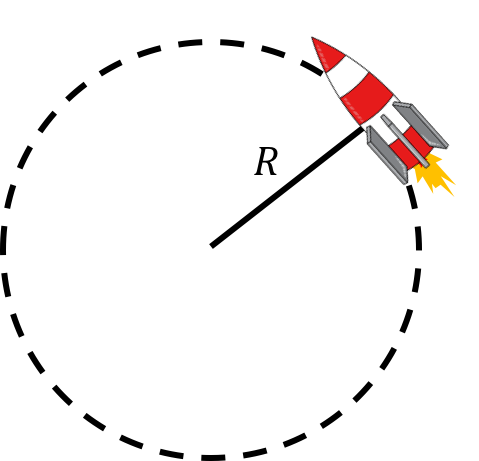
\includegraphics[width=0.375\linewidth]{files/rocket-0b390ecbeda90cfa16a9d338c601a204.png}
\caption[]{A toy rocket accelerating around a circle of radius $R$, as seen from above.}
\label{fig:rotationaldynamics:rocket}
\end{figure}

A toy rocket is attached to a string on a horizontal frictionless table, as shown in Figure~\ref{fig:rotationaldynamics:rocket}. The rocket has a mass $m$ and produces a constant force of thrust with a magnitude $F$ that accelerates the rocket along a circle of radius $R$ (the length of the string). If the rocket starts at rest, what distance along the circumference of the circle will the rocket have travelled after a time, $t$?

\begin{framed}
\textbf{Solution}\\
We can model the rocket as a point particle of mass $m$ with the following forces exerted on it:

\begin{enumerate}
\item $\vec F$, the thrust of the rocket, always acting tangent to the circle.
\item $\vec T$, the force of tension in the string, always acting towards the centre of the circle.
\item $\vec F_g$, the rocket's weight, acting into the page, with magnitude $mg$.
\item $\vec N$, a normal force exerted by the table, out of the page, with magnitude $mg$.
\end{enumerate}

Because the normal force and the weight are equal in magnitude and opposite in direction, the net force will be the sum of the force of thrust and the force of tension, which are always perpendicular to each other. Thinking about this with Newton's Second Law, we could model the force of thrust as increasing the speed of the particle, while the force of tension keeps the rocket moving in a circle (it can do no work to increase the speed, since it is always perpendicular to the motion).

We can also think about this in terms of torques and angular acceleration about the centre of the circle. The thrust will result in a net torque about the centre of rotation, which will lead to the rocket having an angular acceleration. By determining the angular acceleration, we can then model the displacement at some time, $t$, using kinematics. The force of tension will create no torque about the centre of the circle because the force of tension is always co-linear with the position vector, $\vec r$ (the cross-product of co-linear vectors is always zero).

We introduce a coordinate system whose origin coincides with the centre of the circle, as shown in Figure~\ref{fig:rotationaldynamics:rocket_fbd}, so that $\vec r$ corresponds to the position of the rocket relative to the origin.  The force of thrust and the tension are also shown in the diagram. We choose the direction of the $x$ axis such that the rocket was located at the intersection of the $x$ axis and the circle at time, $t=0$.

\begin{figure}[!htbp]
\centering
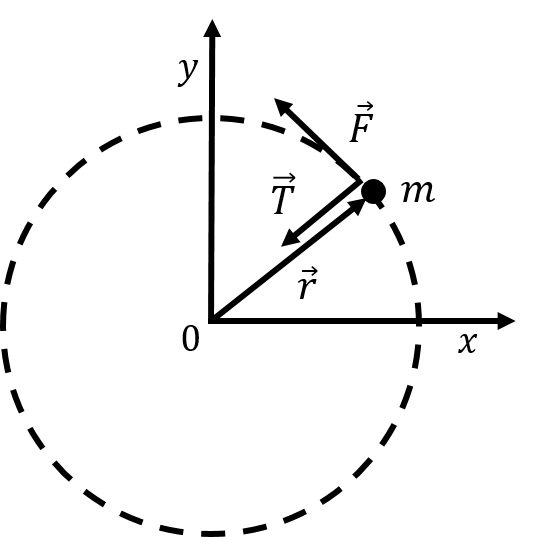
\includegraphics[width=0.375\linewidth]{files/rocket_fbd-9f43c335ae6a2dbd1e2cd746d16b8a55.png}
\caption[]{Coordinate system to describe the motion of the rocket.}
\label{fig:rotationaldynamics:rocket_fbd}
\end{figure}

The net torque on the rocket about the point of rotation is given by the cross-product between the thrust force, $\vec F$, and the position vector, $\vec r$:
\begin{align*}
\vec\tau_{net} = \vec r\times\vec F
\end{align*}
and will point in the positive $z$ direction (as given by the right hand rule). $\vec r$ and $\vec F$ are perpendicular, so the magnitude of the net torque is given by:
\begin{align*}
\tau_{net} = rF \sin(90{\degree}) = RF
\end{align*}
where $R$ is the magnitude of $\vec r$. The net torque vector is thus:
\begin{align*}
\vec\tau_{net} = RF \hat z
\end{align*}
Applying the rotational version of Newton's Second Law allows us to determine the angular acceleration:
\begin{align*}
\vec \tau _{net} &= mr^2\vec\alpha\\
RF \hat z&= mR^2\vec\alpha\\
\therefore \vec \alpha &= \frac{F}{mR}\hat z
\end{align*}
The angular acceleration vector points in the positive $z$ direction (as does the net torque), and indicates that the rocket is accelerating in the counter-clockwise direction about the $z$ axis.

After a period of time $t$, the rocket will have covered an angular displacement, $\Delta \theta$, given by:
\begin{align*}
\Delta \theta &= \theta(t)-\theta_0 = \omega_0t + \frac{1}{2}\alpha t^2\\
&=\frac{1}{2}\frac{F}{mR} t^2
\end{align*}
The linear displacement, $\Delta s$, that corresponds to this angular displacement is:
\begin{align*}
\Delta s = R \Delta\theta = \frac{1}{2}\frac{F}{m} t^2
\end{align*}
\textbf{Discussion:} The formula that we found for the total linear displacement is the same that we would have found if the particle were moving in a straight line with a net force $F$ applied to it (as the particle would have a constant acceleration given by $F/m$).
\end{framed}
\end{framed}

\subsubsection{Torque}\label{sec:rotationaldynamics:torque}

The torque associated with a force is a mathematical tool to describe how much a particular force will cause a particle (or solid) object to rotate about a given point or a given axis of rotation. A torque is \textbf{only defined relative to an axis or point of rotation}. It never makes sense to say ``the torque is ...'', and one should always say "the torque about this axis/point of rotation is ... ". Angular quantities (torque, angular velocity, angular displacement, etc) are only ever defined relative to a specific axis or point of rotation.

Mathematically, the torque vector from a force, $\vec F$, exerted at a position, $\vec r$, relative to the axis or point of rotation is defined as:
\begin{align*}
\vec \tau = \vec r \times \vec F
\end{align*}
Note that the torque from a given force increases if that force is further from the axis of rotation (if $\vec r$ has a bigger magnitude).

Consider the solid disk of radius, $r$, depicted in Figure~\ref{fig:rotationaldynamics:disk}. The disk can rotate about an axis that passes through the centre of the disk and that is perpendicular to the plane of the disk. A force, $\vec F$, is exerted on the edge of the disk as shown.

\begin{figure}[!htbp]
\centering
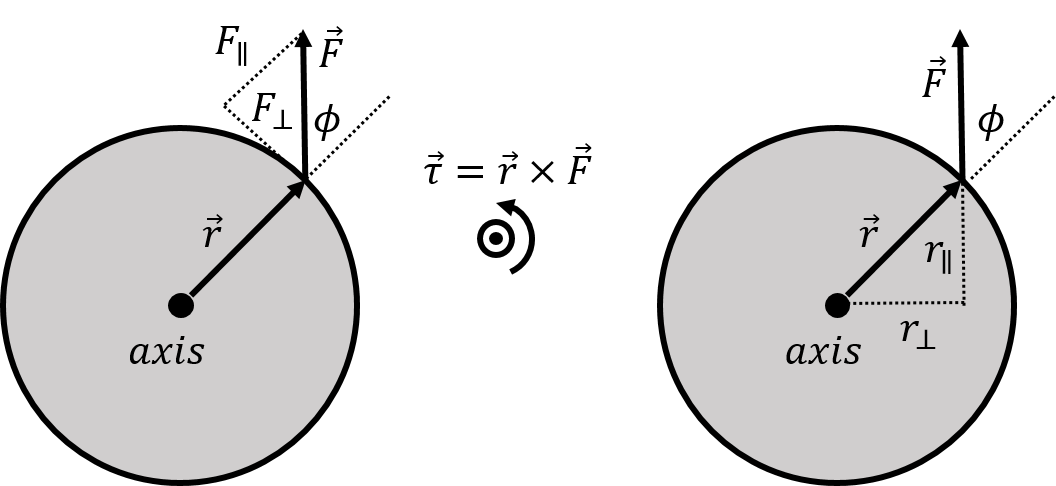
\includegraphics[width=0.625\linewidth]{files/disk-d8d34efd7991e5388b8a772997d35de6.png}
\caption[]{A force exerted on the perimeter of a disk that can rotate about an axis that is perpendicular to the disk and that passes through its centre. We can determine the resulting torque by considering either the component of $\vec F$ that is perpendicular to $\vec r$ (left panel) or the component of $\vec r$ that is perpendicular to $\vec F$ (right panel). The torque vector, $\vec \tau$, is out of the page, as illustrated in the centre.}
\label{fig:rotationaldynamics:disk}
\end{figure}

Intuitively, that force will cause the disk to rotate in the counter-clockwise direction. The torque from the force $\vec F$ about the axis as rotation is given by:
\begin{align*}
\vec \tau = \vec r \times \vec F
\end{align*}
where the vector $\vec r$ is perpendicular to the axis of rotation and goes from the axis of rotation to the point where $\vec F$ is exerted. The direction of the torque vector is out of the page (right hand rule, see Figure~\ref{fig:rotationaldynamics:disk}), and will thus lead to an angular acceleration that is also out of the page, which corresponds to the counter-clockwise direction, as anticipated.

We can break up the force into components that are parallel ($F_\parallel$) and perpendicular ($F_\perp$) to the vector $\vec r$, as shown on the left panel of Figure~\ref{fig:rotationaldynamics:disk}. Only the component of the force that is perpendicular to $\vec r$ will contribute to rotating the disk. Imagine that the force is from a string that you have attached to the perimeter of the disk; if you pull on the string such that the force is parallel to $\vec r$, the disk would not rotate. The magnitude of the torque is given by:
\begin{equation}
\label{eq:rotationaldynamics:taumag}
\tau = rF\sin\phi
\end{equation}
where $\phi$ is the angle between $\vec r$ and $\vec F$, as shown in Figure~\ref{fig:rotationaldynamics:disk}. $F \sin \phi$ is precisely the component of $\vec F$ that is perpendicular to $\vec r$, so we could also write the magnitude of the torque as:
\begin{align*}
\tau =rF_\perp
\end{align*}
which highlights that only the component of the force that is perpendicular to $\vec r$ contributes to the torque. Instead of combining the $\sin \phi$ with $F$ to obtain $F_\perp$, the component of $\vec F$ perpendicular to $\vec r$, we can instead combine the $\sin \phi$ with $r$ in Equation (\ref{eq:rotationaldynamics:taumag}) to obtain $r_\perp$, the component of $\vec r$ that is perpendicular to $\vec F$. This is illustrated in the right panel of Figure~\ref{fig:rotationaldynamics:disk}. The magnitude of the torque is thus also given by:
\begin{align*}
\tau =r_\perp F
\end{align*}
The quantity $r_\perp$ is called the ``lever arm'' of the force about a specific axis of rotation.

\begin{framed}
\textbf{Emma's Thoughts}\\
\textbf{Remembering how to maximize the torque about an axis using a pencil}

We already know that the greater the force that you apply, the more an object will rotate. Here is an easy way to quickly remind yourself of the two other factors that play a role in whether or not an object will rotate:

\textbf{Torque about an axis increases if the force is applied further from the axis of rotation.}

First, pinch the centre of your pencil. Try to make the pencil rotate by pushing right next to where you are pinching. Try making the pencil rotate again, by pushing near the eraser. You should notice that it is much easier to make the pencil rotate by pushing near the eraser, as it is further from the axis of rotation (the pinch).

\textbf{Torque about an axis is maximized if the force is applied perpendicular to the object.}

Next, you should try pushing on the top of the eraser of your pencil, parallel to the pencil. The pencil will not rotate. Now, try pushing on the eraser, but perpendicular to the pencil. In this case, the pencil will rotate.

If you are ever having trouble remembering the factors involved in maximizing torque about an axis, just grab your pencil case and do this quick exercise.
\end{framed}

\begin{framed}
\textbf{Checkpoint}\\
Why is the handle of a door placed on the side of the door that is opposite to the hinges?\}

\begin{enumerate}
\item Because it increases the lever arm of a force used to rotate the door about the handle.
\item Because it increases the perpendicular component of force used to rotate the door about the hinges.
\item Because it increases the lever arm of a force used to rotate the door about the hinges.
\item Because it would be inconvenient if the handle were next to the hinges.
\end{enumerate}

\begin{framed}
\textbf{Answer}\\
\begin{enumerate}[resume]
\item
\end{enumerate}
\end{framed}
\end{framed}

\subsubsection{Rotation about an axis versus rotation about a point}

When defining angular quantities (torque, angular acceleration, etc.), it is important to identify whether these are defined relative to an axis or to a point of rotation. This, in turn, determines the vector $\vec r$ that is involved in the definition of the angular quantities.

Consider a disk of radius $r$ with a force, $\vec F$ exerted on its perimeter, as illustrated in Figure~\ref{fig:rotationaldynamics:fplane}. The disk can only rotate about an axis that is perpendicular to the disk and that goes through the centre of the disk, like a wheel mounted on an axle. The force has a component, $\vec F_{plane}$, that lies in the plane perpendicular to the axis of rotation, and a component, $\vec F_{axis}$, that is parallel to axis of rotation.

\begin{figure}[!htbp]
\centering
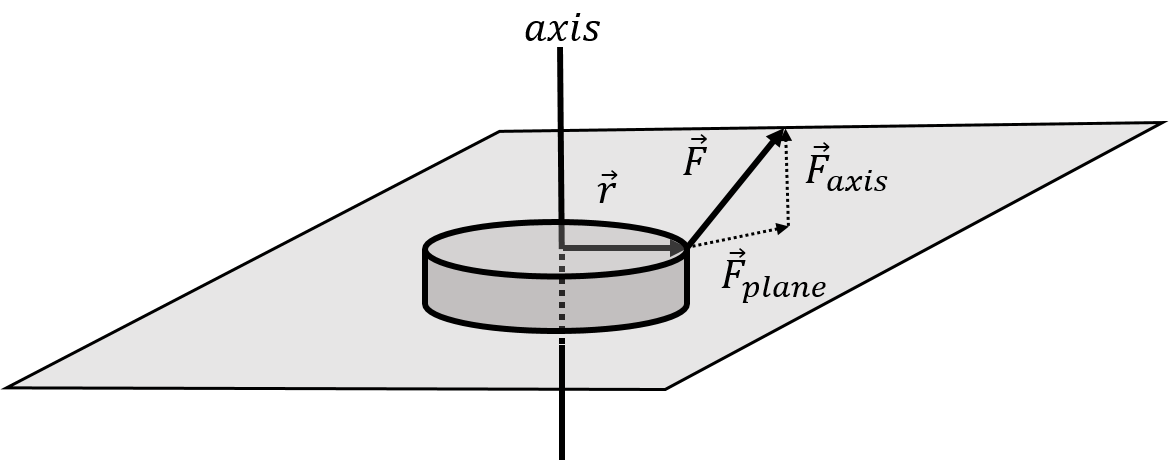
\includegraphics[width=0.625\linewidth]{files/fplane-de1bde47b195b9a91df8497fea637c1f.png}
\caption[]{A force exerted on disk that can only rotate about an axis through its centre and perpendicular to its plane. Only the component of $\vec F$ that is in the plane perpendicular to the axis of rotation, $\vec F_{plane}$, will contribute to the torque about the axis of rotation.}
\label{fig:rotationaldynamics:fplane}
\end{figure}

The vector $\vec r$ is  ** always defined to be perpendicular to the axis of rotation and to go from the axis of rotation to the point where the force $\vec F$ is exerted**, as illustrated. The torque obtained by taking the cross product:
\begin{align*}
\vec \tau = \vec r \times \vec F
\end{align*}
will be perpendicular to both $\vec r$ and $\vec F$, and will thus not be parallel to the axis of rotation. \textbf{Only the component of the torque that is parallel to the axis of rotation} will contribute to rotating the disk about the axis. Only the component of the force that lies in the plane perpendicular to the axis of rotation, $\vec F_{plane}$, will contribute to the component of the torque about that axis of rotation. Thus, when we need to determine the torque about an axis of rotation, we can \textbf{consider vectors $\vec r$ and $\vec F$ that lie in the plane perpendicular to the axis of rotation}. The torque of $\vec F$ relative to the axis of rotation is thus:
\begin{align*}
\vec \tau_{axis} = \vec r \times \vec F_{plane}
\end{align*}
Furthermore, only the component of $\vec F_{plane}$ that is perpendicular to $\vec r$ will contribute to that torque, as we saw in the previous section.

In general, solid objects such as a disk can only rotate about an axis. In that case, one can consider only the components of forces that lie in the plane perpendicular to the axis of rotation in order to calculate the components of the torques about that axis that are parallel to that axis.

A point particle may be able to rotate about any axis that goes through a point of rotation. The net torque vector on the particle about that point will indicate the direction of the axis about which the particle would rotate. This is illustrated in the left panel of Figure~\ref{fig:rotationaldynamics:pointaxis}.

Instead, if the particle were constrained to rotate about the $z$ axis (e.g. if the particle is on a track), then we would use the component of the torque vector that is parallel to the $z$ axis to describe its motion, as illustrated in the right panel. The $z$ component of the torque could be determined by using only the components of the forces that lie in the plane perpendicular to the axis, and defining the vector $\vec r$ from the axis to the particle rather than from the point of rotation to the particle.

\begin{figure}[!htbp]
\centering
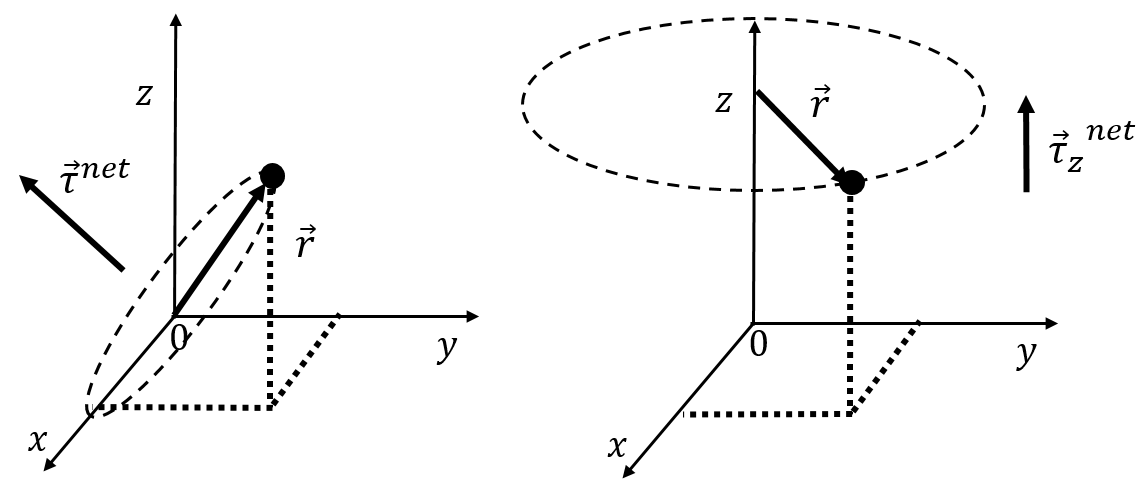
\includegraphics[width=1\linewidth]{files/pointaxis-2f5570c49935cacc05f9e8ef0ae78609.png}
\caption[]{Left panel: a particle rotating about a circle centred at the origin with an axis determined from the net torque vector. Right panel: a particle that is constrained to rotate about the $z$ axis.}
\label{fig:rotationaldynamics:pointaxis}
\end{figure}

\begin{framed}
\textbf{Example 10.2}\\
A force given by $\vec F=F_x\hat x + F_y \hat y + F_z \hat z$ is exerted at a position $\vec r=r_x \hat x + r_y \hat y + r_z\hat z$. Calculate the torque about the $z$ axis as well as the torque about the origin.

\begin{framed}
\textbf{Solution}\\
To calculate the torque about the $z$ axis, we need take the cross-product between the components of the vectors $\vec r$ and $\vec F$ that lie in the $x -y$ plane, since that is the plane perpendicular to the axis of rotation (the $z$ axis). This gives:
\begin{align*}
\vec\tau_z =(r_x \hat x + r_y \hat y) \times (F_x\hat x + F_y \hat y) =(r_xF_y-r_yF_x)\hat z
\end{align*}
If instead we want to calculate the torque about the origin, we take the cross-product between the two vectors:
\begin{align*}
\vec\tau &=(r_x \hat x + r_y \hat y+ r_z\hat z) \times (F_x\hat x + F_y \hat y+ F_z \hat z)\\
&=(r_yF_z-r_zF_y)\hat x+(r_zF_x-r_xF_z)\hat y+(r_xF_y-r_yF_x)\hat z
\end{align*}
If a particle were located at the given position, the force would cause the particle to (instantaneously) rotate about an axis that goes through the origin and is parallel to the torque vector.

\textbf{Discussion:} This example highlights the difference between calculating the torque about an axis of rotation and determining the torque about a point. When calculating the torque about an axis that goes through the origin, we only consider the components of the vectors $\vec r$ and $\vec F$ that are in the plane perpendicular to the axis of rotation. This would correspond to a situation in which the particle is constrained to move in a plane that is perpendicular to the axis of rotation. Instead, if we calculate the torque about the origin, then the torque vector determines the axis of rotation through the origin about which the particle would rotate. In this case, since the axis of rotation is the $z$ axis, and the point of rotation was the origin, the torque about the $z$ axis was simply the $z$ component of the torque calculated about the origin.
\end{framed}
\end{framed}

\subsubsection{Rotational dynamics for a solid object}

We now consider the rotational dynamics for a solid object about a specific axis of rotation. Just as we did in \href{\#momentumandcm}{Chapter 10}, we model a solid object as a system made of many particles of mass $m_i$. Because all of the points in a solid must move in unison, they all \textbf{rotate about an axis of rotation instead of a point}. We describe the position of each particle $i$ by a vector $\vec r_i$ that is \textbf{perpendicular to the axis of rotation and goes from the axis to the corresponding particle}, as shown in Figure~\ref{fig:rotationaldynamics:blob}.

\begin{figure}[!htbp]
\centering
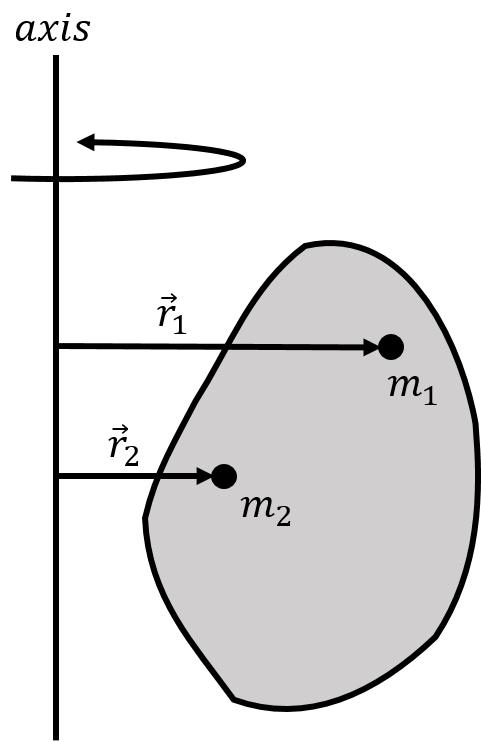
\includegraphics[width=0.375\linewidth]{files/blob-3a7672cec9d414b59409dc409c60ede3.png}
\caption[]{Two point particles that are part of a large solid object and their position vectors relative to an axis of rotation.}
\label{fig:rotationaldynamics:blob}
\end{figure}

We wish to model the motion of the object as it rotates about a specific axis. Thus, when considering the net torque on any particle $i$, we only consider the component of the particle's net torque that is parallel to the axis of rotation (that component of torque that comes from forces that are in the plane perpendicular to the rotation axis).

We can write the rotational version of Newton's Second Law for particle, $i$, with mass $m_i$, and position vector $\vec r_i$ relative to the rotation axis:
\begin{align*}
\sum_k \vec\tau_{ik} = \vec\tau_{i,net} &= m_ir_i^2\vec\alpha_i
\end{align*}
where $\vec\tau_{ik}$ is the $k$-th torque on particle $i$. $\vec\tau_{i,net}$ is the net torque on the particle \textbf{about the axis of rotation} and $\vec\alpha_i$ is the particle's angular acceleration about that axis.

We can divide the torques exerted on a particle into internal and external torques. Internal torques are those exerted by another particle in the system, whereas external torques are exerted by something external to the system. If particle 1 exerts a torque $\vec\tau$ on particle 2, particle 2 will exert an equal and opposite torque, $-\vec\tau$ on particle 1.

Indeed, consider the two particles that exert an equal and opposite force (Newton's Third Law), $\vec F$, on each other, and an arbitrary point/axis of rotation, as illustrated in Figure~\ref{fig:rotationaldynamics:internaltau}. The torque on particle 1 from the force exerted by particle 2 will have the same magnitude as the torque on particle 2 from the force by particle 1. This is because both forces have the same magnitude and they are co-linear, which results in them having the same lever arm. The torque vector from each force will be in opposite directions, because the forces are in opposite direction. Newton's Third Law thus also holds for torques.

\begin{figure}[!htbp]
\centering
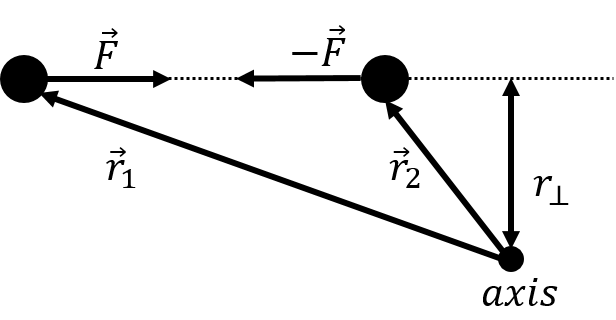
\includegraphics[width=0.375\linewidth]{files/internaltau-7a50341dc6231eb96b051246334dbb8f.png}
\caption[]{Two particles will exert equal and opposite torques on each other due to Newton's Third Law; the forces exerted by each particle on the other are co-linear and will thus have the same lever arm relative to any point/axis of rotation.}
\label{fig:rotationaldynamics:internaltau}
\end{figure}

We can sum together the equations for each particle $i$:
\begin{align*}
\vec\tau_{1,net} + \vec\tau_{2,net} +\vec\tau_{3,net} + \dots &= m_1r_1^2\vec\alpha_1 + m_2r_2^2\vec\alpha_2 +m_3r_3^2\vec\alpha_3 +\dots\\
\sum_i \vec\tau_{i,net} &= \sum_i  m_ir_i^2\vec\alpha_i
\end{align*}
where the sum over all of the torques exerted on each particle will be equal to the net external torque exerted on all of the particles, since the sum of the internal torques, $\vec\tau_{i,int}$, will be zero:
\begin{align*}
\sum_i \vec\tau_{i,net} = \sum_i \vec\tau_{i,int} + \sum_i \vec\tau_{i,ext} = \sum_i \vec\tau_{i,ext} = \vec\tau_{ext}
\end{align*}
where $\vec\tau_{ext}$ is the net external torque on the system.

All of the particles are part of the same rigid body, and cannot move relative to each other. Furthermore, they must all move around circles that are centred about the axis of rotation and in a plane perpendicular to that axis. They must thus all have the same angular acceleration\footnote{They will have different linear accelerations, but the angular acceleration (and angular velocity) will be the same for all particles if they are moving in unison.}, $\vec\alpha_i = \vec \alpha_1 = \vec \alpha_2 =\dots=\vec\alpha$. We can thus factor the angular acceleration, $\vec \alpha$, out of the sum.

We can thus write Newton's Second Law for rotational dynamics of a solid object as:
\begin{align*}
\sum_i \vec\tau_{i,net} &= \sum_i  m_ir_i^2\vec\alpha_i\\
\therefore \vec\tau_{ext}&= \left(\sum_i  m_ir_i^2\right)\vec\alpha
\end{align*}
The term in parentheses describes how the various masses are distributed relative to the axis of rotation. The term in parenthesis is called the \textbf{moment of inertia of the object}, and usually denoted with the letter, $I$:
\begin{equation}
\boxed{I = \sum_i  m_ir_i^2}
\end{equation}
The moment of inertia is a property of the object \textbf{relative to a specific axis of rotation}. Re-writing Newton's Second Law for the rotational dynamics of solid objects using the moment of inertia:
\begin{equation}
\boxed{\vec\tau_{ext} = I\vec\alpha}
\end{equation}
The net torque exerted on an object in the direction of the axis of rotation is thus equal to its moment of inertia about that axis multiplied by its angular acceleration about that axis. In other words, the moment of inertia describes how the object will resist rotational motion given a net torque. An object with a smaller moment of inertia will have a larger angular acceleration for a given torque. Again, this is analogous to the linear case, where the acceleration of an object given a net force is determined by its inertial mass.
ex:rotationaldynamics:dumbbell\_2m)=

\begin{framed}
\textbf{Example 10.3}\\
\begin{figure}[!htbp]
\centering
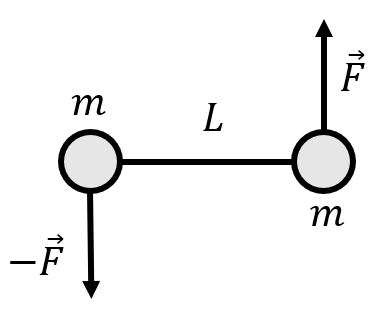
\includegraphics[width=0.375\linewidth]{files/dumbbell_2m-c253a5463337dad4c76ae7e9e9bd51c0.png}
\caption[]{A dumbbell made of two small identical masses separated by a distance $L$.}
\label{fig:rotationaldynamics:dumbbell_2m}
\end{figure}

Two small point masses, $m$, are connected by a mass-less rod of length $L$ to form a dumbbell, as illustrated in Figure~\ref{fig:rotationaldynamics:dumbbell_2m}.
A net force of magnitude $F$ is exerted on each mass, in opposite directions, as illustrated in the Figure.

\begin{enumerate}
\item What is the linear acceleration of the centre of mass of the dumbbell?
\item What is the angular acceleration of the dumbbell relative to an axis that goes through its centre of mass and is perpendicular to the page?
\item What is the angular acceleration of the dumbbell relative to an axis that goes through one of the masses and is perpendicular to the page?
\end{enumerate}

\begin{framed}
\textbf{Solution}\\
We model the dumbbell as a rigid body made of two point masses held at a fixed distance.

\begin{enumerate}
\item The linear acceleration of the centre of mass must be zero, because the net force on the dumbbell is zero. However, just because the centre of mass does not move does not mean that all parts of the dumbbell are immobile.
\item First, we calculate the angular acceleration relative to an axis that is perpendicular the page and goes through the centre of mass. The centre of mass is located midway between the two masses, as illustrated in Figure~\ref{fig:rotationaldynamics:dumbbell_CM}. We also define a coordinate system as shown, such that the $z$ axis is out of the page.
\end{enumerate}

\begin{figure}[!htbp]
\centering
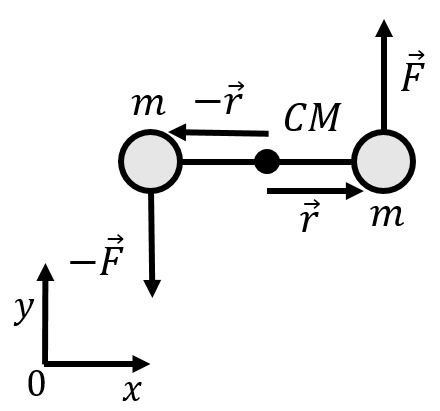
\includegraphics[width=0.375\linewidth]{files/dumbbell_CM-4d677e8005126f5dc3da186bdcf6c161.png}
\caption[]{The dumbbell rotating about the centre of mass.}
\label{fig:rotationaldynamics:dumbbell_CM}
\end{figure}

The vector from the axis of rotation to each mass will have the same magnitude, $r$, but different directions. The net external torque on the dumbbell relative to the axis that goes through the centre of mass, $\vec\tau_{ext}$, which is equal to the sum of the torques from each force:
\begin{align*}
\vec\tau_{ext}&= \vec r \times \vec F + (-\vec r) \times (-\vec F) \\
&= 2 (\vec r \times \vec F)=2 (r\hat x \times F\hat y) = 2rF (\hat x \times \hat y)=2rF\hat z\\
&=LF\hat z
\end{align*}
where we used the fact that $2r = L$. The net torque is thus non zero and in the positive $z$ direction; the dumbbell will have an angular acceleration that is parallel to the net torque, and thus will accelerate in the counter-clockwise direction.

The moment of inertia of the dumbbell relative to the axis through the centre of mass is given by:
\begin{align*}
I = \sum_i  m_ir_i^2 = mr^2 +mr^2 = 2mr^2 = \frac{1}{2}mL^2
\end{align*}
Using Newton's Second Law for rotational dynamics, we find the angular acceleration to be:
\begin{align*}
\vec\tau_{ext}&= I\vec\alpha\\
LF\hat z&=\frac{1}{2}mL^2\vec\alpha\\
\therefore \vec\alpha &= \frac{2F}{mL}\hat z
\end{align*}
Because the centre of mass is fixed (the sum of the forces is zero), the two ends of the dumbbell will rotate about an axis that goes through the centre of mass. This is a feature of all situations in which the net force on an object is zero and the net torque about an axis that goes through the centre of mass is non-zero.

\begin{enumerate}[resume]
\item Let us now calculate the angular acceleration of the dumbbell about an axis that goes through one of the masses, as illustrated in Figure~\ref{fig:rotationaldynamics:dumbbell_end}.
\end{enumerate}

\begin{figure}[!htbp]
\centering
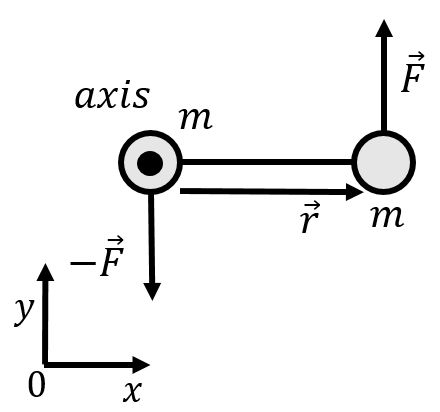
\includegraphics[width=0.375\linewidth]{files/dumbbell_end-097a7e42ada9c2384cb2da98c2b5790a.png}
\caption[]{The dumbbell rotating about one of its ends.}
\label{fig:rotationaldynamics:dumbbell_end}
\end{figure}

We first calculate the net torque on the dumbbell. The vector that goes from the axis of rotation to the force exerted on the mass that coincides with the rotation axis is zero. Thus, only the force exerted on the mass that is not at the rotation axis contributes to the net torque:
\begin{align*}
\vec\tau_{ext}&= \vec r \times \vec F = LF\hat z
\end{align*}
The moment of inertia of the dumbbell about this axis is:
\begin{align*}
I = \sum_i  m_ir_i^2 = m(0)^2 + m(r^2) = mL^2
\end{align*}
which is larger than it was about the centre of mass. Again, the angular acceleration is found using Newton's Second Law for rotational dynamics:
\begin{align*}
\vec\tau_{ext}&= I\vec\alpha\\
LF\hat z&=mL^2\vec\alpha\\
\therefore \vec\alpha &= \frac{F}{mL}\hat z
\end{align*}
We find that the angular acceleration is smaller about an axis that goes through one of the mass than it is about an axis through the centre of mass. Because the centre of mass of the dumbbell is fixed, we can only think of the dumbbell as instantaneously rotating about one of its ends; that is, the motion of the dumbbell will not be such that one mass rotates about the other; this is only true instantaneously.

\textbf{Discussion:} This simple example illustrates several key features about rotational dynamics:

\begin{itemize}
\item If the sum of the forces on an object is zero, it does not mean that the entire object is stationary; it only implies that the centre of mass is stationary (or rather, moving with a constant velocity, but we can always choose to model the system in a frame of reference where the centre of mass is stationary).
\item If the sum of the forces on an object is zero, and the sum of the external torques is non-zero, the object will rotate about an axis that goes through the centre of mass. That is, all points on the object will move along circles that are centred on an axis that goes through the centre of mass.
\item We can model the rotating object about any axis that we choose. In general, the net external torque and the moment of inertia will depend on the choice of axis, as will the resulting angular acceleration.
\item When determining the motion of the centre of mass, we can draw a free-body diagram, and the location of where the forces are exerted do not matter.
\item When determining how the object rotates, we cannot use a free-body diagram, because it matters where the forces are applied (as the torque from a given force depends on the location where the force is applied relative to the axis of rotation).
\end{itemize}
\end{framed}
\end{framed}

\subsubsection{Moment of inertia}

In order to model how an object rotates about an axis, we use Newton's Second Law for rotational dynamics:
\begin{align*}
\vec\tau_{ext} = I \vec \alpha
\end{align*}
where $\vec\tau_{ext}$ is the net external torque exerted on the object about the axis of rotation, $\vec \alpha$ is the angular acceleration of the object, and $I$ is the moment of inertia of the object (about the axis). If we consider the object as being made of many particles of mass $m_i$ each located at a position $\vec r_i$ relative to the axis of rotation, the moment of inertia is defined as:
\begin{align*}
I = \sum_i m_i r_i^2
\end{align*}
Consider, for example, the moment of inertia of a uniform rod of mass $M$ and length $L$ that is rotated about an axis perpendicular to the rod that pass through one of the ends of the rod, as depicted in Figure~\ref{fig:rotationaldynamics:rod}.

\begin{figure}[!htbp]
\centering
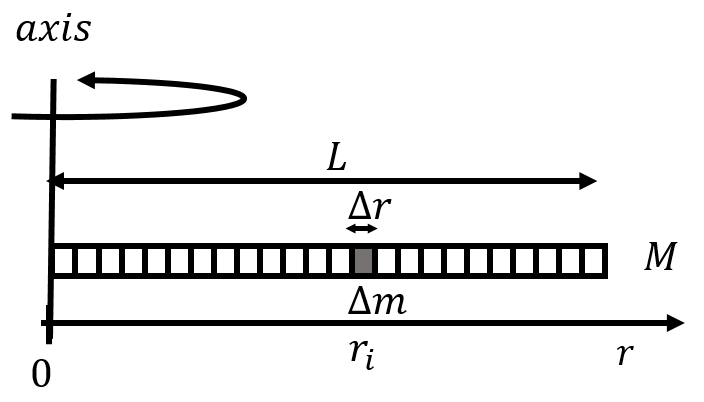
\includegraphics[width=0.375\linewidth]{files/rod-236de0348bd69eedae0f70e34e58fcf2.png}
\caption[]{A rod of length $L$ and mass $M$ being rotated about an axis perpendicular to the rod that goes through one of its ends.}
\label{fig:rotationaldynamics:rod}
\end{figure}

We introduce the linear mass density of the rod, $\lambda$, as the mass per unit length:
\begin{align*}
\lambda = \frac{M}{L}
\end{align*}
We model the rod as being made of many small mass elements of mass $\Delta m$, of length $\Delta r$, at a location $r_i$, as illustrated in Figure~\ref{fig:rotationaldynamics:rod}. Using the linear mass density, the mass element, $\Delta m$, has a mass of:
\begin{align*}
\Delta m = \lambda \Delta r
\end{align*}
The rod is made of many such mass elements, and the moment of inertia of the rod is thus given by:
\begin{align*}
I &= \sum_i \Delta m r_i^2 =\sum_i \left(\lambda \Delta r\right) r_i^2
\end{align*}
If we take the limit in which the length of the mass element is infinitesimally small ($\Delta r \to dr$) the sum can be written as an integral over the dimension of the rod:
\begin{align*}
I &= \int_0^L\lambda r^2dr = \frac{1}{3}\lambda L^3 = \frac{1}{3}\left( \frac{M}{L} \right)L^3 \\
&=\frac{1}{3} ML^2
\end{align*}
where we re-expressed the linear mass density in terms of the mass and length of the rod. In general, we can write the moment of inertia of a continuous object as:
\begin{align*}
I = \int r^2 dm 
\end{align*}
where $dm$ is a small mass element that makes up the object, $r$ is the distance from that mass element to the axis of rotation, and the integral is over the dimension of the object. As we did above, we would usually set up this integral so that $dm$ is expressed in terms of $r$ so that we can take an integral over $r$.

\begin{framed}
\textbf{Example 10.4}\\
Calculate the moment of inertia of a uniform thin ring of mass $M$ and radius $R$, rotated about an axis that goes through its centre and is perpendicular to the disk.

\begin{framed}
\textbf{Solution}\\
We take a small mass element $dm$ of the ring, as shown in Figure~\ref{fig:rotationaldynamics:ring}.

\begin{figure}[!htbp]
\centering
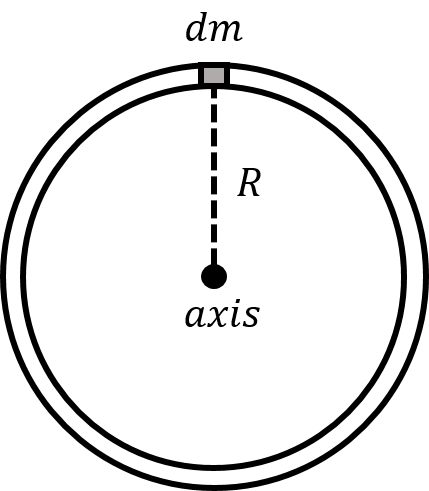
\includegraphics[width=0.375\linewidth]{files/ring-3798bd4dc72f67da8e9c0035c0b3a36e.png}
\caption[]{A small mass element on a ring.}
\label{fig:rotationaldynamics:ring}
\end{figure}

The moment of inertia is given by:
\begin{align*}
I = \int dm r^2
\end{align*}
In this case, each mass element around the ring will be the same distance away from the axis of rotation. The value $r^2$ in the integral is a constant over the whole ring, and so can be taken out of the integral:
\begin{align*}
I = \int dm r^2 = R^2\int dm
\end{align*}
where we used the fact that the ring has a radius $R$, so the distance $r$ of each mass element to the axis of rotation is $R$. The integral:
\begin{align*}
\int dm
\end{align*}
just means ``sum all of the mass elements, $dm$'', and is thus equal to $M$, the total mass of the ring. The moment of inertia of the ring is thus:
\begin{align*}
I = R^2\int dm = MR^2
\end{align*}
\end{framed}
\end{framed}

\paragraph{The parallel axis theorem}

The moment of inertia of a solid object can be difficult to calculate, especially if the object is not symmetric. The parallel axis theorem allows us to determine the moment of inertia of an object about an axis, if we already know the moment of inertia of the object about an axis that is parallel and goes through the centre of mass of the object.

Consider an object for which we know the moment of inertia, $I_{CM}$, about an axis that goes through the object's centre of mass. We define a coordinate system such that the origin is located at the centre of mass, and the $z$ axis is parallel to the axis about which we know the moment of inertia, as illustrated in Figure~\ref{fig:rotationaldynamics:parallel}.

\begin{figure}[!htbp]
\centering
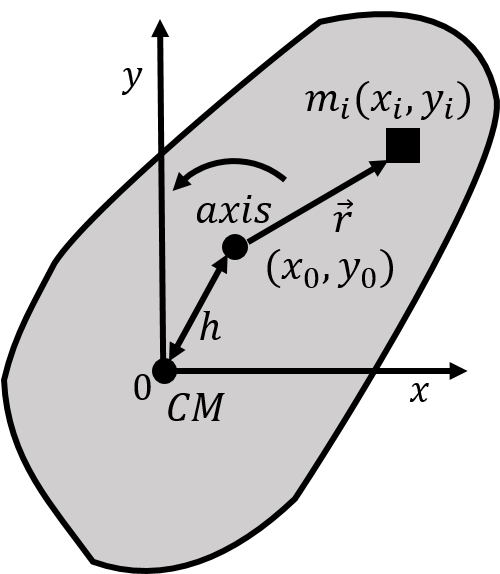
\includegraphics[width=0.375\linewidth]{files/parallel-d3ee8a85ea4e4e83cbf6748bc4b31764.png}
\caption[]{An object with a coordinate system whose origin is at the object's centre of mass, and for which we know the moment of inertia about the $z$ axis. We wish to determine the object's moment of inertia through a second axis, parallel to the $z$ axis, but located a distance $h$ away from the centre of mass.}
\label{fig:rotationaldynamics:parallel}
\end{figure}

We wish to determine the moment of inertia for the object for an axis that is parallel to the $z$ axis, but goes through a point with coordinates $(x_0,y_0)$ located a distance $h$ away from the centre of mass. The moment of inertia about an axis parallel to the $z$ axis and that goes through that point, $I_h$ is given by:
\begin{align*}
I_h = \sum_i m_i r_i^2
\end{align*}
where $m_i$ is a mass element of the object located at a distance $r_i$ from the axis of rotation. If the mass element is located at a position $(x_i,y_i)$ relative to the centre of mass, we can write the distance $r_i$ in terms of the position of the mass element, and of the position of the axis of rotation:
\begin{align*}
r_i^2 = (x_i-x_0)^2+(y_i-y_0)^2 = x_i^2-2x_ix_0+x_0^2+y_i^2-2y_iy_0+y_0^2
\end{align*}
Note that:
\begin{align*}
x_0^2 + y_0^2 = h^2
\end{align*}
The moment of inertia, $I_h$, can thus be written as:
\begin{align*}
I_h &= \sum_i m_i r_i^2 =\sum_i (m_i(x_i^2+ y_i^2)-2x_0m_ix_i-2y_0m_iy_i+m_ih^2)\\
&=\sum_i m_i(x_i^2+ y_i^2) + h^2\sum_i m_i - 2x_0 \sum_im_ix_i- 2y_0 \sum_im_iy_i
\end{align*}
where we broke the sum up into several sums, and factored constant terms ($h$, $x_0$, $y_0$) out of the sums, since these constants do not depend on which mass element we are considering. The first term is the moment of inertia about the centre of mass, since $x_i^2+y_i^2$ is the distance to the centre of mass. The second term is $h^2$ times the total mass of the object, since the sum of all the $m_i$ is just the mass, $M$, of the object. Now consider the term:
\begin{align*}
-2x_0 \sum_im_ix_i
\end{align*}
The sum, $\sum m_i x_i$ is the numerator in the definition of the $x$ coordinate of the centre of mass! The sum is thus zero, because we choose the origin to be located at the centre of mass. The last two terms in the sum are thus identically zero, because they correspond to the $x$ and $y$ coordinates of the centre of mass!

We can thus write the parallel axis theorem:
\begin{equation}
\boxed{I_h = I_{CM} + Mh^2}
\end{equation}
where $I_{CM}$ is the moment of inertia of an object of mass $M$ about an axis that goes through the centre of mass and, $I_h$, is the moment of inertia about a second axis that is parallel to the first and a distance $h$ away.

\begin{framed}
\textbf{Example 10.5}\\
In the previous section, we calculated the moment of inertia of a rod of length $L$ and mass $M$ through an axis that is perpendicular to the rod and through one of its ends, and found that it was given by:
\begin{align*}
I=\frac{1}{3}ML^2
\end{align*}
What is the moment of inertia of the rod about an axis that is perpendicular to the rod and goes through its centre of mass?

\begin{framed}
\textbf{Solution}\\
In this case, we know the moment of inertia through an axis that does not go through the centre of mass. The centre of mass is located a distance $h=L/2$ away from the point about which we know the moment of inertia, $I_h$.

Using the parallel axis theorem, we can find the moment of inertia through the centre of mass:
\begin{align*}
I_{CM} &= I_h - Mh^2\\
&=\frac{1}{3}ML^2 - M \left( \frac{L}{2}\right)^2 = \frac{1}{12}ML^2
\end{align*}

\textbf{Discussion:} We find that the moment of inertia about the centre of mass is smaller than the moment of inertia about the end of the rod. This makes sense because when rotating the rod about its end, more of its mass is further away from the axis of rotation, which results in a larger moment of inertia.
\end{framed}
\end{framed}

\subsubsection{Equilibrium}

In this section, we consider the conditions under which an object is in static or dynamic equilibrium. An object is in equilibrium if it does not rotate when viewed in a frame of reference where the object's centre of mass is stationary (or moving at constant velocity).

\paragraph{Static equilibrium}

An object is in static equilibrium, if \textbf{both the sum of the external forces exerted on the object and the sum of the external torques (about any axis) are zero}. If the object is in static equilibrium the centre of mass will have no acceleration and the object will have no angular acceleration. In the centre of mass frame of reference, the object is immobile.

\begin{framed}
\textbf{Example 10.6}\\
\begin{figure}[!htbp]
\centering
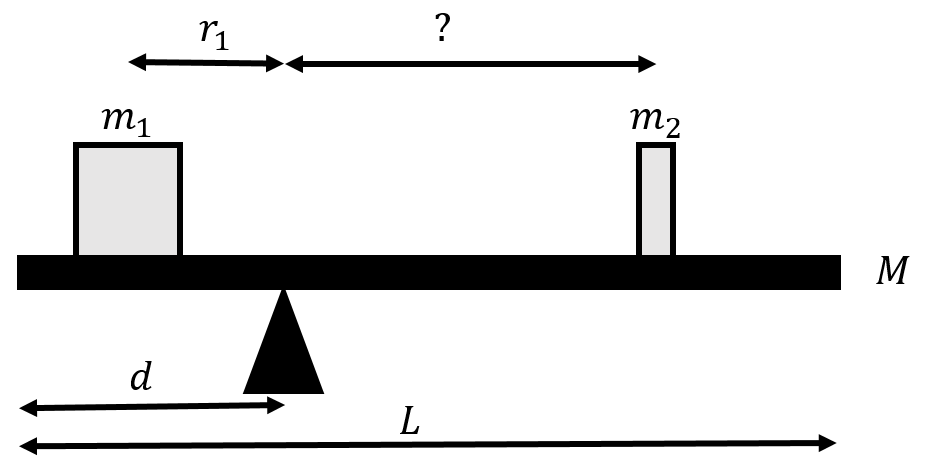
\includegraphics[width=0.625\linewidth]{files/scale-7513564151b88bb65ea62810e588cb41.png}
\caption[]{Two masses on a balance.}
\label{fig:rotationaldynamics:scale}
\end{figure}

Two masses, $m_1$ and $m_2$ are placed on a balance as shown in Figure~\ref{fig:rotationaldynamics:scale}. The balance is made of a plank of mass $M$ and length $L$ that is placed on a fulcrum that is a distance $d$ from one of the edges of the plank. If mass $m_1$ is placed at a distance $r_1$ from the fulcrum, how far should mass $m_2$ be placed on the other side of the plank in order for the balance to be in equilibrium?

\begin{framed}
\textbf{Solution}\\
We can consider the plank as the object that is in static equilibrium. Thus, the sum of the forces and the sum of the torques on the plank must be zero. We first start by identifying the forces that are exerted on the plank; these are:

\begin{enumerate}
\item $\vec F_g$, the weight of the plank, exerted at the centre of mass of the plank.
\item $\vec F_1$, a force equal to the weight of mass $m_1$, exerted at the location of $m_1$.
\item $\vec F_2$, a force equal to the weight of mass $m_2$, exerted at the location of $m_2$.
\item $\vec N$, a normal force exerted by the fulcrum.
The forces are illustrated in Figure~\ref{fig:rotationaldynamics:scale_fbd} along with our choice of coordinate system. The $z$ axis is not illustrated, and is directed out of the page.
\end{enumerate}

\begin{figure}[!htbp]
\centering
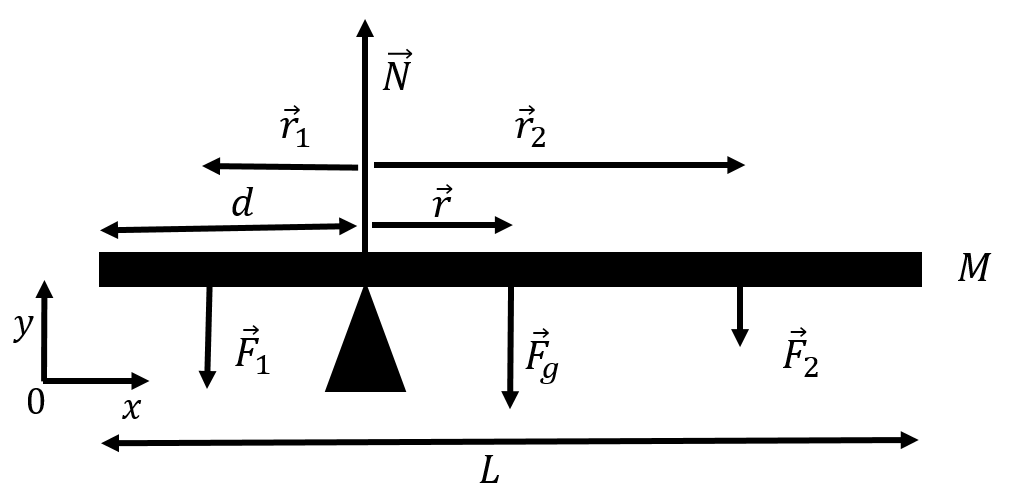
\includegraphics[width=0.375\linewidth]{files/scale_fbd-6fe39975f4790393f62e15e2de0cb66f.png}
\caption[]{Forces exerted on the plank.}
\label{fig:rotationaldynamics:scale_fbd}
\end{figure}

All of the forces are in the $y$ direction, so we only write the $y$ component of Newton's Second Law (with zero acceleration), which allows us to determine the magnitude of the normal force:
\begin{align*}
\sum F_y = N - Mg -m_1g - m_2 g &=0\\
\therefore N &= (M+m_1+m_2) g
\end{align*}

Because the plank is in static equilibrium, the sum of the torques must also be zero. We can choose the axis of rotation about which to calculate the torques. We choose an axis that is parallel to the $z$ axis (out of the page) and goes through the fulcrum. In general, since we can choose the axis of rotation, it is usually convenient to choose an axis that goes through a point where at least one force is being exerted, because the torque from that force will be zero (its lever arm will be zero).  Furthermore, since all of the forces are in the $xy$ plane, the net torque on the plank will be in the $z$ direction, so it makes sense to choose an axis in that direction.

The torques from the weight of the plank and from the force exerted by mass $m_2$ will be in the negative $z$ direction, and the torque from the force exerted by mass $m_1$ will be in the positive $z$ direction. The normal force will not result in any torque, because it is exerted at the axis of rotation and has a lever arm of zero.

We define $\vec r_1$ as the vector from the fulcrum to mass $m_1$. The torque, $\vec \tau_1$, from the force exerted by mass $m_1$ is given by:
\begin{align*}
\vec \tau_1 &= \vec r_1 \times \vec F_1 = (-r_1 \hat x) \times (-F_1 \hat y) \\
&= r_1F_1(\hat x \times \hat y) = r_1F_1\hat z=r_1m_1g\hat z
\end{align*}
where we used the fact that the magnitude of $\vec F_1$ is $m_1 g$. Similarly, the torques from the force exerted by $m_2$, $\vec\tau_2$, and by the weight, $\vec\tau_g$, are given by:
\begin{align*}
\vec \tau_2 &=\vec r_2 \times \vec F_2 = -m_2 g r_2 \hat z\\
\vec \tau_g &=\vec r \times \vec F_g=-rMg\hat z = -\left(\frac{L}{2}-d\right)Mg\hat z
\end{align*}
where $\frac{L}{2} -d$ is the distance between the fulcrum and where the weight of the plank is exerted. We require that the $z$ component of the net torque be equal to zero (since all of the torques are in the $z$ direction), which allows us to determine $r_2$:
\begin{align*}
\sum \tau_z = \tau_{1z} + \tau_{2z} + \tau_{gz} &=0\\
m_1 g r_1 -m_2 g r_2 -\left(\frac{L}{2}-d\right)Mg &=0\\
\therefore r_2 = \frac{1}{m_2} \left(m_1r_1-\left(\frac{L}{2}-d\right)M\right)
\end{align*}
Note that because we chose to calculate the torques about a point that goes through the fulcrum, in this case, we did not need to determine the value of the normal force which we obtained from Newton's Second Law.

\textbf{Discussion:} This example highlights the fact that when an object is in static equilibrium, we can choose a convenient axis about which to calculate the torques. In this case, by calculating the torques about the fulcrum, we did not need to consider the torque from the normal force. If we had chosen a different point, then the torque from the normal force would have been non-zero, and we would have used Newton's Second Law to express the normal force in terms of the other quantities. Physically, if we had placed the fulcrum at the centre of the plank $d = L/2$, then we would have found that $m_1r_1 = m_2r_2$, the well known equation for a balance. This equation, of course, comes from requiring that the torques from the forces exerted by $m_1$ and $m_2$ are equal in magnitude and opposite in direction.
\end{framed}
\end{framed}

\paragraph{Dynamic equilibrium}

\begin{framed}
\textbf{Review}\\
Before proceeding, you may wish to review Section~\ref{sec:newtonslaws:inertialforces} on inertial forces.
\end{framed}

When an object is in dynamic equilibrium, its centre of mass is accelerating, but the object is not rotating when viewed from its centre of mass frame of reference. Thus, the sum of the external forces exerted on the object is not zero, while the net external torque exerted on the object is zero, in the frame of reference of the centre of mass.

Consider, for example, a speed skater going around a circular track of radius $R$, and leaning into the centre making an angle $\theta$ with the ice, as depicted in Figure~\ref{fig:rotationaldynamics:skater}. The skater's centre of mass is accelerating, because she is going around a circle, so the net force on the skater is not zero. However, in the reference frame of the skater, the skater is not rotating; she is thus in dynamic equilibrium.

\begin{figure}[!htbp]
\centering
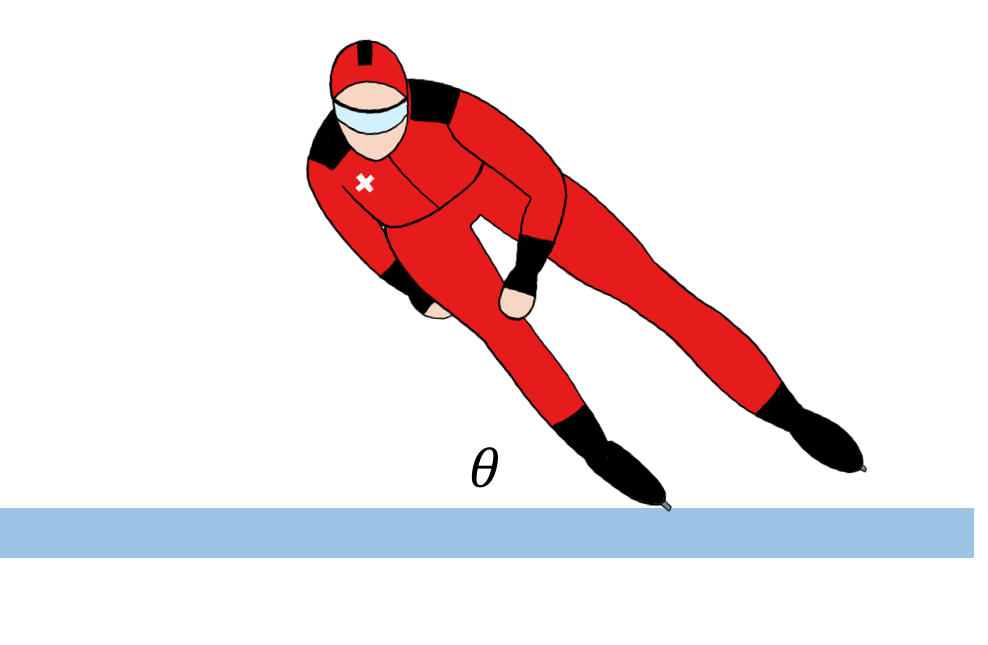
\includegraphics[width=0.625\linewidth]{files/skater-de5ef9789e4b98b933c3d897130ba429.png}
\caption[]{A speed skater leaning in as she goes around a circle.}
\label{fig:rotationaldynamics:skater}
\end{figure}

The forces on the skater are:

\begin{enumerate}
\item $\vec F_g$, her weight, exerted at her centre of mass with magnitude, $Mg$.
\item $\vec N$, a normal force, exerted by the ice upwards on her skates.
\item $\vec f_s$, a force of static friction, exerted towards the centre of the circle, by the ice on her skates.
\end{enumerate}

The forces are illustrated in Figure~\ref{fig:rotationaldynamics:skater_fbd} along with our choice of coordinate system.

\begin{figure}[!htbp]
\centering
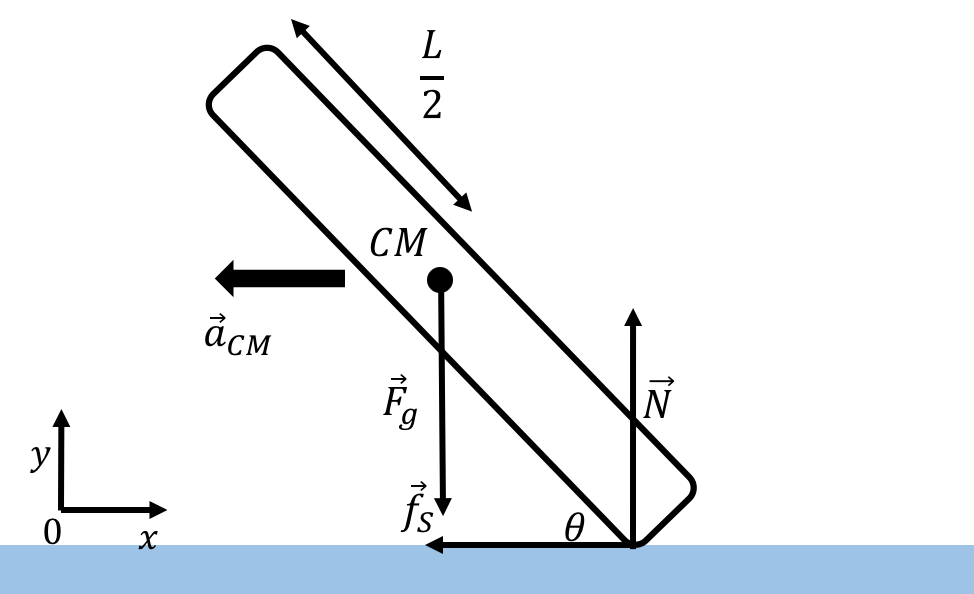
\includegraphics[width=0.625\linewidth]{files/skater_fbd-98c8ebbab45d9c93cc3a6b544de6d1e2.png}
\caption[]{Forces on the speed skater from Figure~\ref{fig:rotationaldynamics:skater}.}
\label{fig:rotationaldynamics:skater_fbd}
\end{figure}

The sum of the forces exerted on the skater must be towards the centre of the circle and equal to the mass of the skater times her centripetal acceleration (which is the acceleration of her centre of mass, $\vec a_{CM}$). The $x$ and $y$ components of Newton's Second Law are thus given by:
\begin{align*}
\sum F_x &= -f_s = -ma_{CM} = m\frac{v^2}{R}\\
\sum F_y &= N-mg = 0
\end{align*}

All of the forces exerted on the skater are in the $xy$ plane, so we consider torques about an axis that is co-linear with the $z$ axis. Consider the torques about an axis through the point of contact between the skates and the ice; there is a net torque in the counter-clockwise direction due to the weight of the skater (the weight is the only force that can result in a torque about the point of contact with the ice). We expect that the skater would topple over, however, this must not be a correct model for the skater, since we know that it is possible for her to lean in without falling.

Consider, instead, the sum of the torques about an axis through her centre of mass. If the skater has a length $L$ and the centre of mass is in the middle of the skater, the sum of the torques about the centre of mass is given by the torques from the normal forces and the force of friction:
\begin{align*}
\sum \tau = \tau_{Nz} + \tau_{f_sz} = \frac{L}{2}\cos\theta N - \frac{L}{2}\sin\theta f_s
\end{align*}
About the centre of mass, the torques must be zero for the skater not to rotate, and this would give a relation between the force of static friction and the normal force.

Why do we get an incorrect model when we take the torques about the point of contact between the ice and the skater? In order to determine if the skater is rotating, we need to be in the same reference frame as the skater. However, the frame of reference of the skater is not an inertial frame of reference, since the skater is accelerating. We can still model the forces on the skater in the non-accelerating frame of reference, \textbf{as long as we include the inertial force, $-m\vec a_{CM}$}, in that frame of reference. In the frame of reference of the skater, there is an additional inertial force, $-m\vec a_{CM}$, in order for the sum of the forces to be zero (in the frame of reference of the skater, the sum of the forces must be zero since the skater is not accelerating in that frame of reference). The additional inertial force is exerted at the centre of mass, as illustrated in Figure~\ref{fig:rotationaldynamics:skater_fbdcm}.

\begin{figure}[!htbp]
\centering
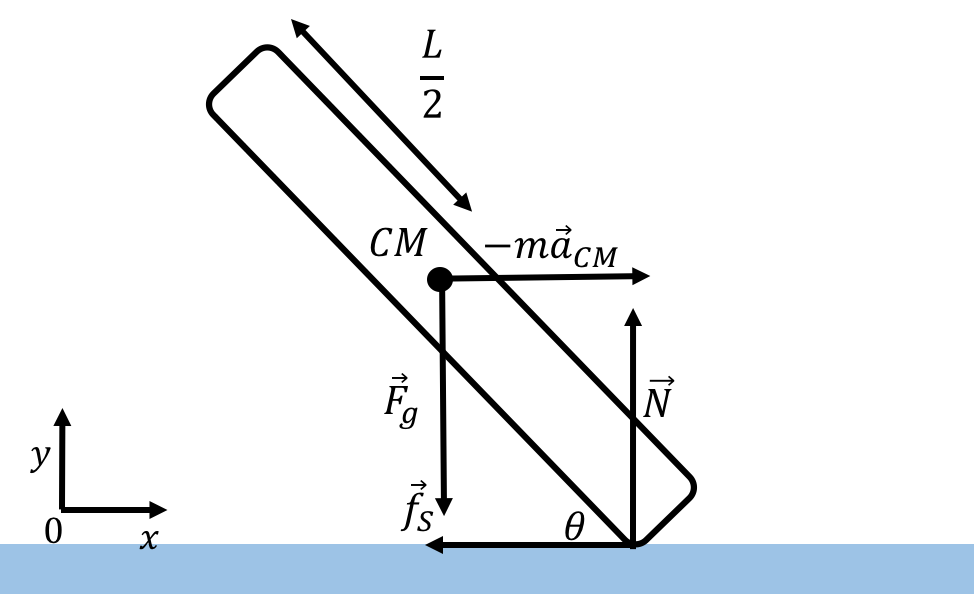
\includegraphics[width=0.625\linewidth]{files/skater_fbdcm-216251e49c689969b105377acad7e7bb.png}
\caption[]{Forces on the speed skater from Figure~\ref{fig:rotationaldynamics:skater} as seen in the accelerating frame of reference of the centre of mass.}
\label{fig:rotationaldynamics:skater_fbdcm}
\end{figure}

The reason that our model worked when taking the torques about the centre of mass is that the inertial force, exerted at the centre of mass, does not result in a torque (since it has a lever arm of zero). Our model was technically wrong, but if we take the torques about the centre of mass, then we do not need to worry about the inertial force. If we include the additional inertial force, then we can take the torques about any point, just as in the static equilibrium case.

\subsubsection{Summary}

We can describe the kinematics of rotational motion using vectors to indicate both an axis of rotation and the direction of rotation about that axis. If a particle with velocity vector, $\vec v$, is rotating in an circle about an axis, then its angular velocity vector, $\vec\omega$, relative to that axis is defined as:
\begin{align*}
\vec\omega = \frac{1}{r^2}\vec r \times \vec v
\end{align*}
where $\vec r$ is a vector from the axis of rotation to the particle. The particle rotates in a circle that lies in the plane defined by $\vec r$ and $\vec v$, perpendicular to the axis of rotation. The direction of the angular velocity vector is co-linear with the axis of rotation and the direction of rotation is given by the right-hand rule for axial vectors.

One can define the angular velocity of a particle relative to a point of rotation, even if the particle is not moving in a circle. In that case, the angular velocity corresponds to the angular velocity of the particle as if it were instantaneously moving about a circle.

If a particle moving around a circle has a tangential acceleration, $\vec a_s$, then its angular acceleration vector is defined as:
\begin{align*}
\vec\alpha = \frac{1}{r^2}\vec r \times \vec a_s
\end{align*}

The torque from a force, $\vec F$, exerted at a position $\vec r$, relative to an axis (or point) of rotation is defined as:
\begin{align*}
\vec\tau &= \vec r \times \vec F\\
\end{align*}
Torque is analogous to force in that it is used to model the causes of motion. Torques are only ever defined relative to an axis or point of rotation. The torque vector will be co-linear with the axis about which the object on which the force is exerted would rotate as a result of that force.

The magnitude of the torque can be written using either the component of the force, $F_\perp$ perpendicular to the vector $\vec r$, or the lever arm, $r_\perp$, of the force relative to the axis of rotation:
\begin{align*}
\tau &= rF\sin\phi\\
&=rF_\perp\\
&=r_\perp F
\end{align*}
where $\phi$ is the angle between the vectors $\vec r$ and $\vec F$ when these are placed ``tail to tail''.

Using rotational/angular quantities, we can modify Newton's Second Law to describe rotational dynamics about a given axis (or point) of rotation. For a point particle, this gives:
\begin{align*}
\vec \tau_{net} = mr^2 \vec\alpha
\end{align*}
where $\vec \tau_{net}$ is the net torque on the particle (the sum of the torques from each force exerted on the particle) about the axis, and $\vec\alpha$ is the resulting angular acceleration about that axis.

For an object (either continuous or made of point particles), the rotational version of Newton's Second Law for rotation about a specific axis is given by:
\begin{align*}
\vec \tau_{net} = I\vec\alpha
\end{align*}
where $I$ is the moment of inertia of the object about that axis.

The moment of inertia of an object about an axis of rotation is given by
\begin{align*}
I = \sum_i m_ir_i^2
\end{align*}
if the object is modelled as a system of point particles of mass $m_i$ each a distance $r_i$ from the axis of rotation. For a continuous object, the moment of inertia is given by:
\begin{align*}
I = \int r^2 dm
\end{align*}
where $dm$ is a small mass element a distance $r$ from the axis of rotation and the integral is over the dimension of the object. Generally, one can set up the integral by expressing $dm$ in terms of $r$ using the density of the object, and then integrating $r$ over the dimension of the object.

If the moment of inertia of an object of mass $M$ about an axis that goes through the centre of mass is given by $I_{CM}$, then the moment of inertia, $I_h$, of the object through an axis that is parallel and a distance $h$ from the centre of mass is given by the parallel axis theorem:
\begin{align*}
I_h = I_{CM} + Mh^2 \quad \text{Parallel axis theorem}
\end{align*}

Objects are in equilibrium if they are not rotating when viewed in their centre of mass frame of reference. Thus, for an object to be in equilibrium, the sum of the torques on the object, in the centre of mass reference frame, must be zero.

An object is in static equilibrium if the centre of mass is not accelerating, and thus the sum of the external forces on the object is zero. To model the torques on an object in static equilibrium, one can choose the axis about which to calculate the torques. A good choice is to choose an axis that is perpendicular to the plane in which the forces on the object are exerted (if such a plane exists), and to choose the axis to go through a point where at least one force is exerted (so that torques exerted at that point are identically zero).

An object is in dynamic equilibrium if the centre of mass is accelerating, but the object does not rotate when viewed in the frame of reference of its centre of mass. In dynamic equilibrium, if one models the torques exerted on the object about an axis that does not go through the centre of mass, then one must remember to include an inertial force exerted at the centre of mass.

\begin{framed}
\textbf{Important Equations}\\
\bigskip\noindent
\begin{tabular}{p{\dimexpr 0.500\linewidth-2\tabcolsep}p{\dimexpr 0.500\linewidth-2\tabcolsep}}
\toprule
 &  \\
\hline
\textbf{Angular Quantities} & \textbf{Newton's Second Law for a point particle about a given axis of rotation} \\
$\vec\omega = \frac{1}{r^2}\vec r \times \vec v\\$ $\vec\alpha = \frac{1}{r^2}\vec r \times \vec a_\perp\\$ $\vec v_s = \vec \omega \times \vec r\nonumber\\$ $\vec a_s = \vec \alpha \times \vec r$ & $\vec \tau_{net} = mr^2 \vec\alpha\\$ \\
\textbf{Torque from a force} & \textbf{Newton's Second Law for rotation about an axis} \\
$\vec\tau = \vec r \times \vec F\\$ $\tau = rF\sin\phi\\$ $\tau=rF_\perp\\$ $\tau=r_\perp F$ & $\vec \tau_{net} = I\vec\alpha$ \\
\textbf{Parallel Axis Theorem} & \textbf{Moment of Inertia} \\
$I_h = I_{CM} + Mh^2$ & $I = \sum_i m_ir_i^2\\$ $I = \int r^2 dm$ \\
\bottomrule
\end{tabular}

\bigskip
\end{framed}

\begin{framed}
\textbf{Important Definitions}\\
\textbf{Torque:} A rotational equivalent of force which occurs when a force is applied at a distance $r$ from the axis of rotation of a rigid body or particle. SI units: $\left[\text{J}\right]$. Common variable(s): $\tau$.

\textbf{Moment of inertia:} A property of matter which describes an object's resistance to rotational motion. SI units: $\left[ \text{kg}\cdot\text{m}^2\right]$. Common variable(s): $I$.

\textbf{Linear mass density:} The mass per unit length of an object. SI units: $\left[\text{kg}\cdot \text{m}^{ -1}\right]$. Common variable(s): $\lambda$.
\end{framed}

\subsubsection{Thinking about the material}

\begin{framed}
\textbf{Reflect and research}\\
\begin{itemize}
\item Compare the steering wheels of a small car and a large transport truck. What are the differences, and why?
\item List 2 kitchen utensils that use torque to ``get the job done''.
\end{itemize}
\end{framed}

\begin{framed}
\textbf{To try at home}\\
\begin{itemize}
\item Take a large textbook and consider the 3 axes that are parallel to the sides of the textbook and go through the centre of mass. By rotating the book along the three axes successively, determine the axis about which the moment of inertia of the textbook is the largest.
\item Confirm that the moment of inertia of a rod is smaller if the rod is rotated about its centre of mass than if it is rotated by one of its ends.
\end{itemize}
\end{framed}

\begin{framed}
\textbf{To try in the lab}\\
\begin{itemize}
\item Propose an experiment to measure the moment of inertia of an object and to compare that to a model prediction.
\item Construct a comeback can, then model the forces which make the toy's peculiar motion possible.
\end{itemize}
\end{framed}

\subsubsection{Sample problems and solutions}

\paragraph{Problems}

\begin{framed}
\textbf{Problem 10.1}\\
Calculate the moment of inertia of a uniform disk of mass $M$ and radius $R$, rotated about an axis that goes through its centre and is perpendicular to the disk.
\end{framed}

\begin{framed}
\textbf{Problem 10.2}\\
\begin{figure}[!htbp]
\centering
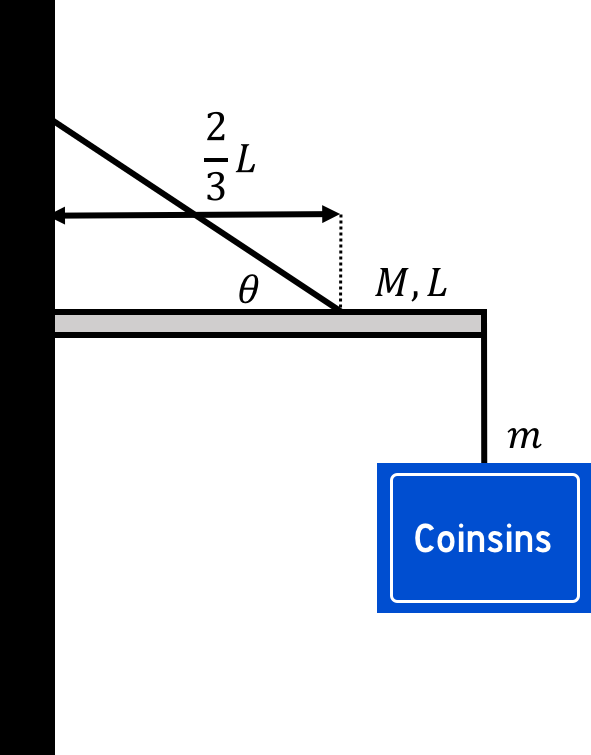
\includegraphics[width=0.375\linewidth]{files/sign-93ec4d5e525231b8707d63b708054088.png}
\caption[]{sign is suspended on a horizontal bar of mass $M$ and length $L$.}
\label{fig:rotationaldynamics:sign}
\end{figure}

A sign holder is built by attaching a bar of mass $M$ and length $L$ to a wall using a hinge that allows the bar to rotate in the vertical plane. The sign of mass $m$ is attached to the end of the  bar that is opposite fo the wall. The bar is held up by a rope that is attached to the wall on one end and to the bar on the other end, two thirds of the length of the bar from the wall, as illustrated in Figure~\ref{fig:rotationaldynamics:sign}. The rope makes an angle $\theta$ with respect to the horizontal bar. Find the tension in the rope and the magnitude of the force exerted by the hinge onto the bar.
\end{framed}

\paragraph{Solutions}

\begin{framed}
\textbf{Solution 10.1}\\
We need to split up the disk into mass elements, $dm$, that we can sum together to obtain the moment of inertia of the disk. We can choose a ring of radius $r$ and radial thickness $dr$ for the shape of our mass element, as depicted in Figure~\ref{fig:rotationaldynamics:diskI}.

\begin{figure}[!htbp]
\centering
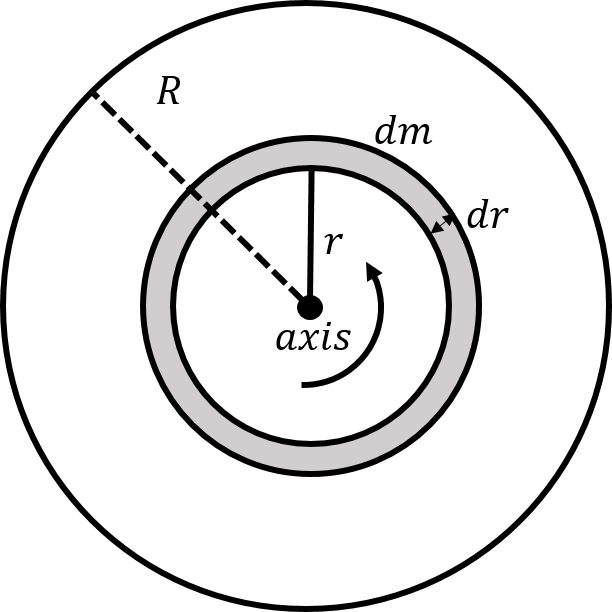
\includegraphics[width=0.375\linewidth]{files/diskI-cde410e1a6a2ec40a14e7e5e216d4893.png}
\caption[]{A mass element, $dm$, in the shape of a ring of radius $r$ and radial thickness $dr$.}
\label{fig:rotationaldynamics:diskI}
\end{figure}

We can define a surface mass density, $\sigma$, equal to the mass per unit area of the disk:
\begin{align*}
\sigma = \frac{M}{\pi R^2}
\end{align*}
The mass of the ring shaped element is thus given by:
\begin{align*}
dm = \sigma 2\pi r dr
\end{align*}
where $2\pi r dr$ is the area of the mass element. You can imagine unfolding the mass element into a rectangle of height $dr$ and of length $2\pi r$ to obtain its area. Now that we have expressed the mass element in terms of $r$, we can proceed to calculate the moment of inertia of the disk.

We know from the Example~10.4, that the infinitesimal moment of inertia, $dI$, of a ring of radius $r$ and infinitesimal mass, $dm$, about its axis of symmetry is given by:
\begin{align*}
dI = dm r^2
\end{align*}

The moment of inertia of the disk, is found by summing the moments of inertia of the infinitesimal rings:
\begin{align*}
I &=\int dI = \int dm r^2 = \int_0^R \sigma 2\pi r dr r^2 =2\pi \sigma \int_0^R  r^3 dr \\
&=2 \pi \sigma \frac{1}{4}R^4 = 2\pi \left( \frac{M}{\pi R^2} \right) \frac{1}{4}R^4\\
&=\frac{1}{2}MR^2
\end{align*}
where we removed the surface mass density by expressing it in term of the total mass and radius of the disk.

\textbf{Discussion:} The moment of inertia of a disk of mass $M$ and radius $R$ is half of that of a ring of radius $R$ and mass $M$. It is thus easier to rotate the disk than the ring.
\end{framed}

\begin{framed}
\textbf{Solution 10.2}\\
The whole system does not move and so it is in static equilibrium. In order to determine the forces exerted on the bar by the rope and the hinge, we model the bar as being in static equilibrium. The forces exerted on the bar are:

\begin{itemize}
\item $\vec F_g$, the weight of the bar, with magnitude $Mg$, exerted at the bar's centre of mass.
\item $\vec F_m$, a downwards forced exerted by the sign at the end of the bar, with magnitude $mg$.
\item $\vec T$, a force of tension exerted by the rope at a distance $2/3 L$ from the wall.
\item $\vec R$, a force exerted by the hinge on the bar at the end next to the wall\footnote{We chose the letter R for ``Reaction'', as this is the force of reaction from the hinge as the bar pushes against the hinge.}. We expect that the force from the hinge will have both a horizontal component, $R_x$, and a vertical component, $R_y$, in order for the net force on the bar to be zero.
\end{itemize}

The forces are illustrated in Figure~\ref{fig:rotationaldynamics:sign_fbd} along with our choice of coordinate system (and the $z$ axis, not shown, points out of the page).

\begin{figure}[!htbp]
\centering
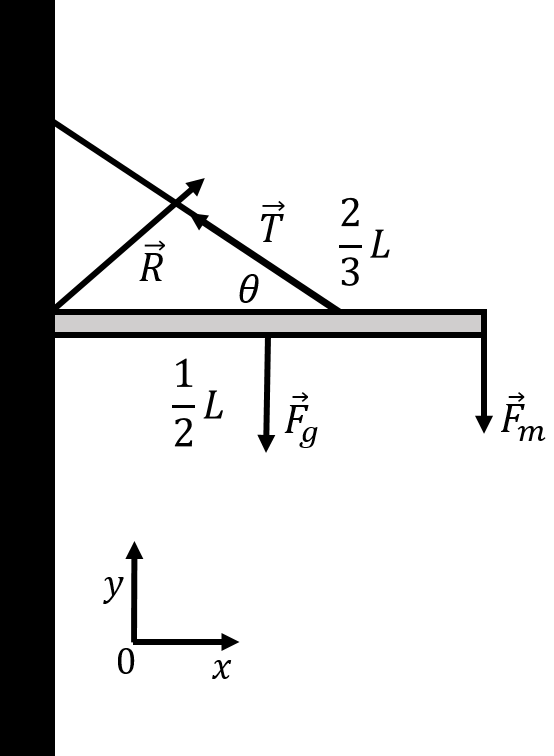
\includegraphics[width=0.375\linewidth]{files/sign_fbd-ffe4168e450dcf3dc23b6bf92f8cb8c1.png}
\caption[]{Forces on the bar that is holding the sign of mass $m$.}
\label{fig:rotationaldynamics:sign_fbd}
\end{figure}

We start by writing out the $x$ and $y$ components of Newton's Second Law (with zero acceleration):
\begin{align*}
\sum F_x &= R_x - T\cos\theta =0\\
\sum F_y &= R_y + T\sin\theta - Mg - mg=0
\end{align*}
We can choose the axis about which to calculate the torques. Since all of the forces are in the $xy$ plane, we choose to calculate the torques about an axis parallel to the $z$ axis that goes through the hinge on the wall. The force from the hinge, $\vec R$, will thus result in a torque of zero (since it has a lever arm of zero). The torque from each force about the hinge is given by:
\begin{align*}
\vec \tau_M &= \vec r_M \times \vec F_g = \left(\frac{L}{2}\hat x\right) \times (-Mg \hat y) =-Mg\frac{L}{2} \hat z\\
\vec \tau_T &= \vec r_T \times \vec T = \left(\frac{2}{3}L\hat x\right) \times (-T\cos\theta \hat x + T\sin\theta \hat y) =\frac{2}{3}LT\sin\theta \hat z\\
\vec \tau_m &= \vec r_m \times \vec F_m = (L\hat x) \times (-mg \hat y) =-mgL\hat z\\
\end{align*}
The sum of the torques in the $z$ direction must be zero for static equilibrium, which allows us to determine the magnitude of the force of tension:
\begin{align*}
\sum \tau_z = \tau_{Mz} + \tau_{Tz}+ \tau_{mz} &=0\\
-Mg\frac{L}{2} + \frac{2}{3}LT\sin\theta -mgL &=0\\
-Mg\frac{1}{2} + \frac{2}{3}T\sin\theta -mg &=0\\
\therefore T&= \frac{3g}{2\sin\theta} \left( m + \frac{M}{2}\right)
\end{align*}
Using the $x$ and $y$ components of Newton's Second Law, we can now use the tension to determine the $x$ and $y$ components of the force exerted by the hinge:
\begin{equation}
R_x &= T\cos\theta = \frac{3g}{2\tan\theta} \left( m + \frac{M}{2}\right)\\
R_y &= (M+m)g - T\sin\theta = (M+m)g - \frac{3}{2}g \left( m + \frac{M}{2}\right)=  \left( \frac{1}{4}M-\frac{1}{2}m\right)g
\end{equation}
We find that the $y$ component of the force from the hinge could be in the positive or negative $y$ direction, depending on the sign of $\left( \frac{1}{4}M -\frac{1}{2}m\right)$. In particular, if $M>2m$, then the force exerted by the hinge, $\vec R$, has a component in the positive $y$ direction, as illustrated in Figure~\ref{fig:rotationaldynamics:sign_fbd}. However, if $M<2m$, then the hinge exerts a force that has a negative component in the $y$ direction, unlike that illustrated in the Figure.

\textbf{Discussion:} In this example, we saw that we needed to use both the sum of the forces and the sum of the torques in order to determine the forces on the bar.
\end{framed}